%!TEX root = ../3dchapter.tex

\setchapterpreamble[u]{\margintoc}

\graphicspath{{mat/}}

\chapter{The Medial Axis Transform}%
\label{chap:mat}

The Medial Axis Transform (MAT) is yet another way to represent a 3D model.
It can be considered a \emph{dual} representation to the b-rep, similar to how the Voronoi diagram is dual to the Delaunay triangulation. 
Contrary to the b-rep, that represents a model by describing explicitly its boundary surface, the MAT describes a model by its \emph{skeleton} (compare Figures~\ref{fig:gbm:brep} and \ref{fig:gbm:maxis}).
Both the MAT and the b-rep contain exactly the same information and it is possible to convert one to the other without loss of information.

Compared to other shape representations, this skeleton structure makes different properties of the model explicit.
For example, the MAT allows us to split a shape into parts simply by looking at the branches of the skeleton. 
The resulting shape parts often turn out to be meaningful in practice. 
Observe for instance that for the gingerbread man in Figure~\ref{fig:gingerman}, its arms, legs, torso and head each have one corresponding branch in its medial axis (compare Figures~\ref{fig:gbm:whole} and \ref{fig:gbm:maxis}).
For DTMs for example, equally meaningful decompositions into parts can be made, \eg\ the MAT allows us to decompose a DTM into separate hills, watercourses and other objects on top the DTM (see Figure~\ref{fig:matterrain}).

\section{Defining the MAT}
The MAT can be computed both for 2D and 3D objects (compare Figures~\ref{fig:3dmat_2d} and~\ref{fig:3dmat_halfopen}).
\begin{figure}
	\centering
	\begin{subfigure}[b]{0.25\linewidth}
		\centering
		
\includegraphics[width=\textwidth]{figs/gingerbreadman_whole.pdf}
		\caption{A 2D object}
		\label{fig:gbm:whole}
	\end{subfigure}
	\qquad%
	\begin{subfigure}[b]{0.25\linewidth}
		\centering
		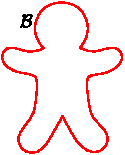
\includegraphics[width=\textwidth]{figs/gingerbreadman_brep.pdf}
		\caption{b-rep}
		\label{fig:gbm:brep}
	\end{subfigure}
	\qquad%
	\begin{subfigure}[b]{0.25\linewidth}
		\centering
		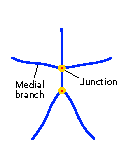
\includegraphics[width=\textwidth]{figs/gingerbreadman_skeleton.pdf}
		\caption{Interior MAT}
		\label{fig:gbm:maxis}
	\end{subfigure}
	
	\begin{subfigure}[b]{0.3\linewidth}
		\centering
		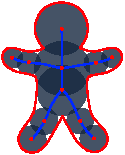
\includegraphics[width=\textwidth]{figs/gingerbreadman_mat.pdf}
		\caption{b-rep + MAT with medial balls}
		\label{fig:gbm:mballs}
	\end{subfigure}
	\qquad
	\begin{subfigure}[b]{0.3\linewidth}
		\centering
		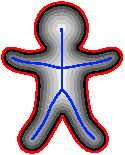
\includegraphics[width=\textwidth]{figs/gingerbreadman_grassfire.pdf}
		\caption{b-rep + contours of equal distance to it + MAT}
		\label{fig:gbm:dt}
	\end{subfigure}
	
	\caption{Different ways to represent the shape of gingerbread man}
	\label{fig:gingerman}
\end{figure}
\begin{figure}
	\centering
	\begin{subfigure}{0.26\linewidth}
		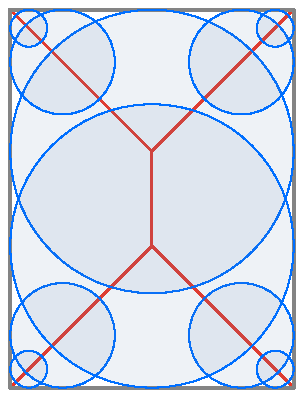
\includegraphics[width=\linewidth]{figs/Box2D3D/3dmat_2d.pdf}
		\subcaption{The MAT for a 2D box consists of medial balls (blue) and the medial axis (red).}
		\label{fig:3dmat_2d}
	\end{subfigure}
	\quad
	\begin{subfigure}{0.33\linewidth}
		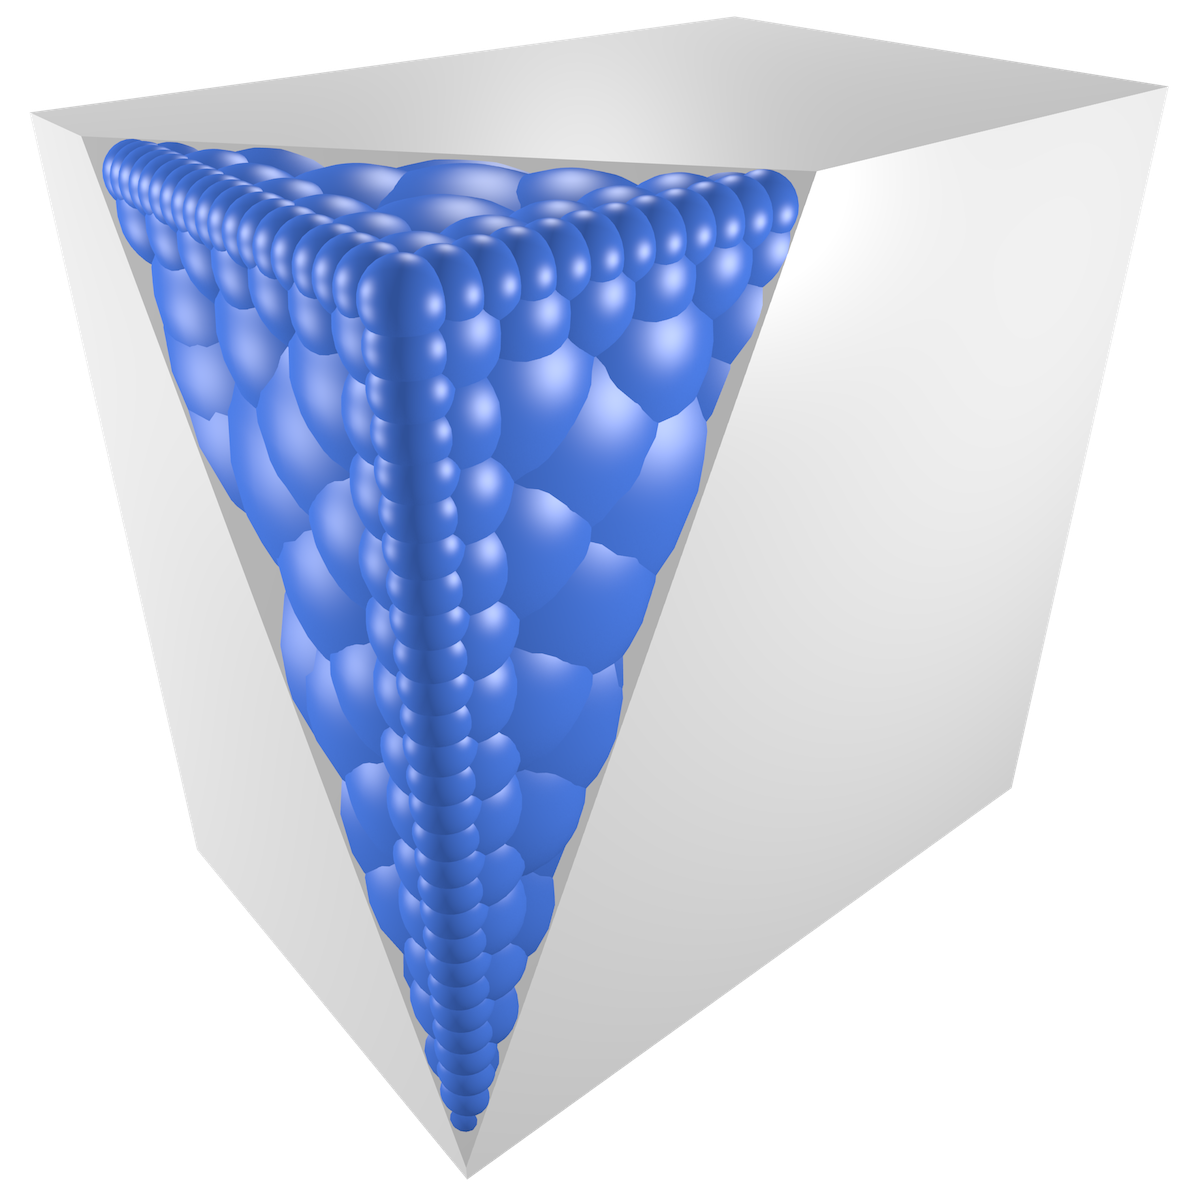
\includegraphics[width=\linewidth]{figs/Box2D3D/3dmat_halfopen.png}
		\subcaption{3D medial balls of a 3D box shape.}
		\label{fig:3dmat_halfopen}
	\end{subfigure}
	\quad
	\begin{subfigure}{0.33\linewidth}
		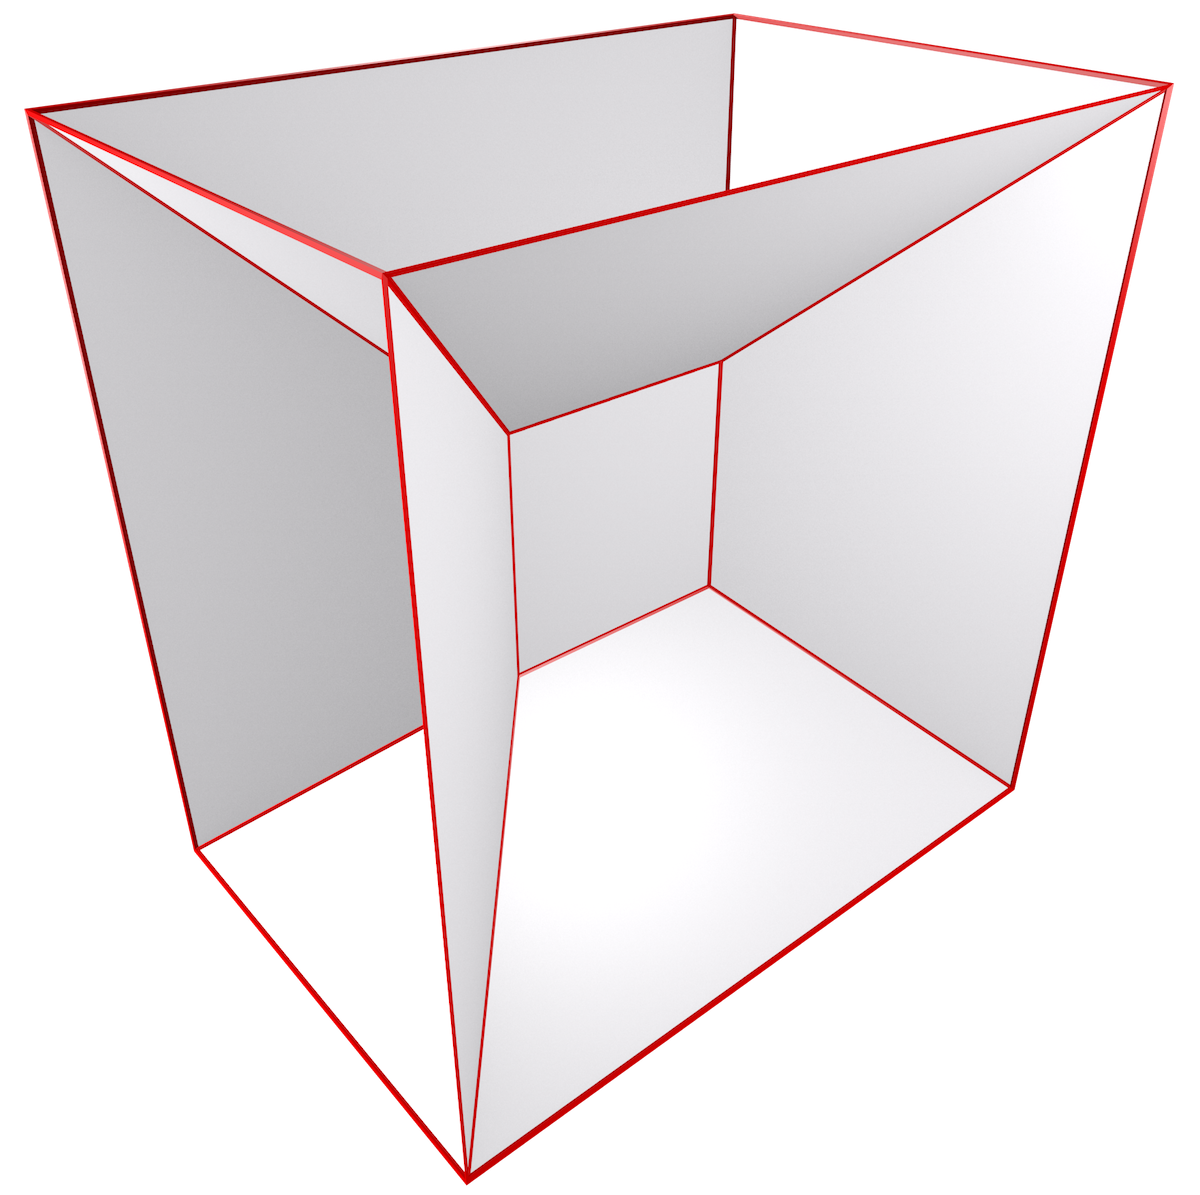
\includegraphics[width=\linewidth]{figs/Box2D3D/3dmat_sheets.png}
		\subcaption{3D medial axis of a 3D box shape.}
		\label{fig:3dmat_sheets}
	\end{subfigure}
	\caption{The MAT in 2D and in 3D for a box shape.}
	\label{fig:3dmat}
\end{figure}
In both cases there are two equivalent definitions of the MAT\footnote{Sometimes the MAT is referred to as medial axis function, stick figure, skeleton or surface skeleton.
	Inventor Harry Blum finally settled on symmetry axis, as he considered symmetry to be the crucial role of the MAT \citep{Blum73}.} that apply. 
One is based on the distance transform, and one is based on medial balls. 
Both definitions describe how to obtain the MAT from the boundary, denoted $
\mathcal{B}$ of an object (Figure~\ref{fig:gbm:brep}).
And both can be applied to both 2D and 3D objects .

\begin{description}
	\item[Grassfire analogy]
	Imagine that everything is made of grass and that all the points on $\mathcal{B}$ are simultaneously set on fire at time $t=0$. 
	The fire spreads evenly to all directions at constant speed. 
	Now, the MAT is defined as the set of points where the fire front meets itself. 
	This concept is illustrated in Figure~\ref{fig:gbm:dt}, where each contour can be seen as a fire front at some constant time $t$. The medial axis is drawn where the fire front meets itself.
	\item[Medial balls]
	A \emph{medial ball} is a ball that fits completely inside $\mathcal{B}$ and does not contain any other ball that would fit inside $\mathcal{B}$. 
	The MAT is defined as the set of points that are the centres of all medial balls of $\mathcal{B}$ (see Figure~\ref{fig:gbm:mballs}). 
	Notice that each medial ball touches $\mathcal{B}$ in at least two points, called its \emph{feature points}. 
\end{description}

%TODO: that should also be in the figure
As illustrated in Figure~\ref{fig:gbm:maxis}, the MAT can be subdivided into \emph{medial branches} and \emph{junctions}. 
Junctions are locations where three or more medial branches coincide. 
The points of the MAT are called \emph{medial atoms}, or simply \emph{atoms}. 
Observe that if an atom has exactly two feature points, it is part of a medial branch, and if it has more than two feature points it lies on a junction or on the tip of a medial branch. 
The medial branches, its junctions and how those are are connected define the \emph{medial structure}.
% If we consider that each branch corresponds to one part of $\mathcal{B}$ gives us a natural way to split an object into parts

For a 2D object, such as in Figure~\ref{fig:gingerman}, the medial branches are curves and the the junctions are points. 
However, for a 3D object, the medial branches can also be surfaces (see Figure~\ref{fig:3dmat_sheets}), and the junctions can also be curves.
The branches of the 3D MAT are therefore also called \emph{medial sheets}.

\subsection{Medial geometry}
The medial geometry describes how atoms are related to the object boundary $\mathcal{B}$. 
It is defined for each medial atom that is part of a medial sheet. 
Figure~\ref{fig:medialgeometry} illustrates the complete medial geometry of an atom.
The medial ball $B$ has the atom $\mathbf{c}$ at its center and has a radius $r$, \ie\ the shortest distance from $\mathbf{c}$ to $\mathcal{B}$.
The medial ball $B$ touches the boundary $\mathcal{B}$ at the feature points $\mathbf{p}$ and $\mathbf{q}$.
The vectors from $\mathbf{c}$ to $\mathbf{p}$ and $\mathbf{q}$ are called the \emph{spoke vectors}, denoted $\vec{\mathbf{s_{p}}}$ and $\vec{\mathbf{s_{q}}}$. 
The angle between the spoke vectors is called the \emph{separation angle}, denoted $\theta$ and the bisector of the spoke vectors is called the \emph{medial bisector}, denoted $\vec{\mathbf{b}}$.

\begin{figure}
	% \centering
	% \setcapindent{1em}
	\centering
	\begin{minipage}[c]{0.4\linewidth}
		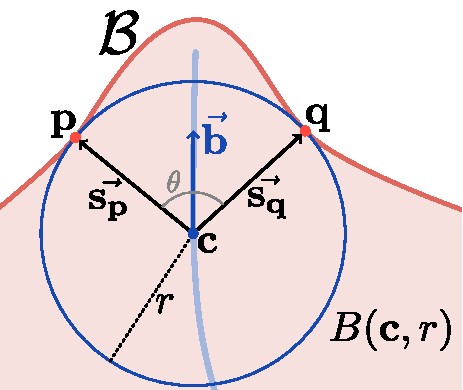
\includegraphics[width=\linewidth]{figs/medial_atom_geometry.pdf}
	\end{minipage}
	\begin{minipage}[c]{0.45\textwidth}
		% \hspace{1.1em}
		\centering
		\begin{tabular}{ll}
			\toprule
			Symbol & Description \\
			\midrule
			$B(\mathbf{c},r)$& medial ball\\
			$\mathbf{c}$ & medial atom\\
			$r$ & radius\\
			$\mathbf{p}, \mathbf{q}$ & feature points\\
			$\vec{\mathbf{s_{p}}}, \vec{\mathbf{s_{q}}}$ & spoke vectors\\
			$\theta$ & separation angle\\
			$\vec{\mathbf{b}}$ & medial bisector\\
			\bottomrule
		\end{tabular}
	\end{minipage}
	\caption{The geometry of a medial atom.}
	\label{fig:medialgeometry}
\end{figure}

% maximal/medial ball, primary and secondary feature point, primary and secondary medial ball, separation angle, bisector, medial atom:point+ball+metrics, 
% defining local coordinate system
% \subsection{Properties of the MAT}
Using the medial geometry we can describe a number of interesting properties of the MAT.
\begin{enumerate}
	\item Any atom $\mathbf{c}$ is always \emph{medial} to $\mathcal{B}$, \ie\ it is equidistant to the feature points of $\mathbf{c}$ (hence the name of the MAT).
	\item The medial ball $B$ is always tangential to $\mathcal{B}$ at the feature points. 
	\item The radius $r$ can be used to define the `thickness' of an object, since it measured the distance to the `middle' of the object where the MAT is located.
	% \item From the union of all interior medial balls of an object, its boundary can be reconstructed.
	% \item The medial bisector $\vec{\mathbf{b}}$ always points in the direction of decreasing radius along a medial branch or sheet.
	% \item The feature points of a medial atom at the tip of a medial branch indicate points of minimal of curvature on $\mathcal{B}$. Notice also that the radius of those atoms is inversely proportional to the curvature at its feature points.
\end{enumerate}

\subsection{Exterior MAT and the MAT of a DTM}
The MAT can be divided into an interior part and an exterior part.
So far we have only looked at the \emph{interior MAT}, which consists of medial balls that reside entirely on the inside of an object.
However, in many cases it is also possible to define medial balls that reside entirely on the outside of an object.
That part of the MAT is called the \emph{exterior MAT}.
An object can only have an exterior MAT if the shape of that object is non-convex, since for convex object it is not possible to find exterior medial balls with a finite radius.
% In case of a composition of multiple objects, the interaction between these object can also lead to an exterior MAT, even if all objects are convex.\todo{illustrate that}

The separation between inside and outside is very clear and unambiguous for a an object with a closed boundary such as the gingerbread man of Figure~\ref{fig:gingerman} or for any perfectly manifold boundary.
However, for objects that are not completely closed this separation is less clear, as there could be MAT sheets that connect the interior and exterior parts though holes in the boundary surface.
In some cases with an open boundary a reasonable distinction can still be made.
For example for a DTM we can follow the convention that the `ground side` of the DTM is the interior, and the `sky side' is the exterior, as follows from Figure~\ref{fig:object_earth}.
\begin{figure}
	\centering
	\begin{subfigure}{0.4\linewidth}
		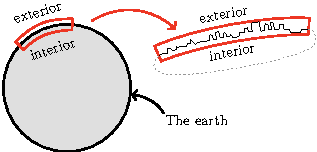
\includegraphics[width=\linewidth]{figs/object_earth.pdf}
		\subcaption{The interior and exterior of a DTM.}
	\label{fig:object_earth}
	\end{subfigure}
	\quad
	\begin{subfigure}{0.57\linewidth}
		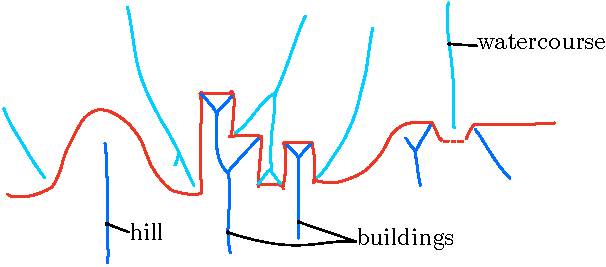
\includegraphics[width=\linewidth]{figs/MAT_hierarchy.pdf}
		\subcaption{For a terrain the MAT is typically subdivided into open clusters that correspond to features such as hills, buildings and watercourses in the terrain. Shown here is a vertical cross section of a DTM. Exterior MAT in light blue, interior MAT in dark blue.}
		\label{fig:matterrain}
	\end{subfigure}
	\caption{Defining interior and exterior for an open surface such as a terrain.}
	\label{fig:intext}
\end{figure}
Following this convention, we can still define the interior and exterior MAT of a DTM, see for instance Figure~\ref{fig:matterrain}.

\subsection{Medial clusters}
The interior and exterior MAT can consist of multiple disjoint parts (\eg\ in Figure~\ref{fig:matterrain}).
For closed objects the interior MAT is always one part, whereas the exterior MAT can be multiple parts depending on the number of concavities in the object boundary.
The disjoint parts are called \emph{medial clusters}.
Each medial cluster is in fact a set of adjacent sheet where each adjacency is also a junction between medial sheets.

For objects with open boundaries like DTMs, there can also be multiple interior medial clusters.
In this case one object on the terrain typically corresponds to one medial cluster (Figure~\ref{fig:matterrain}).
Figure~\ref{fig:smat_r3d_int} also illustrates how the MAT can thus be used to meaningfully subdivide an object into parts.
For an input that is simply a surface point cloud that happens to contain several object, we can detect easily these objects by looking at the medial clusters of its MAT.
This effectively decomposes the object into meaningful sub-objects.
\begin{figure}
	\begin{subfigure}[t]{0.45\linewidth}
		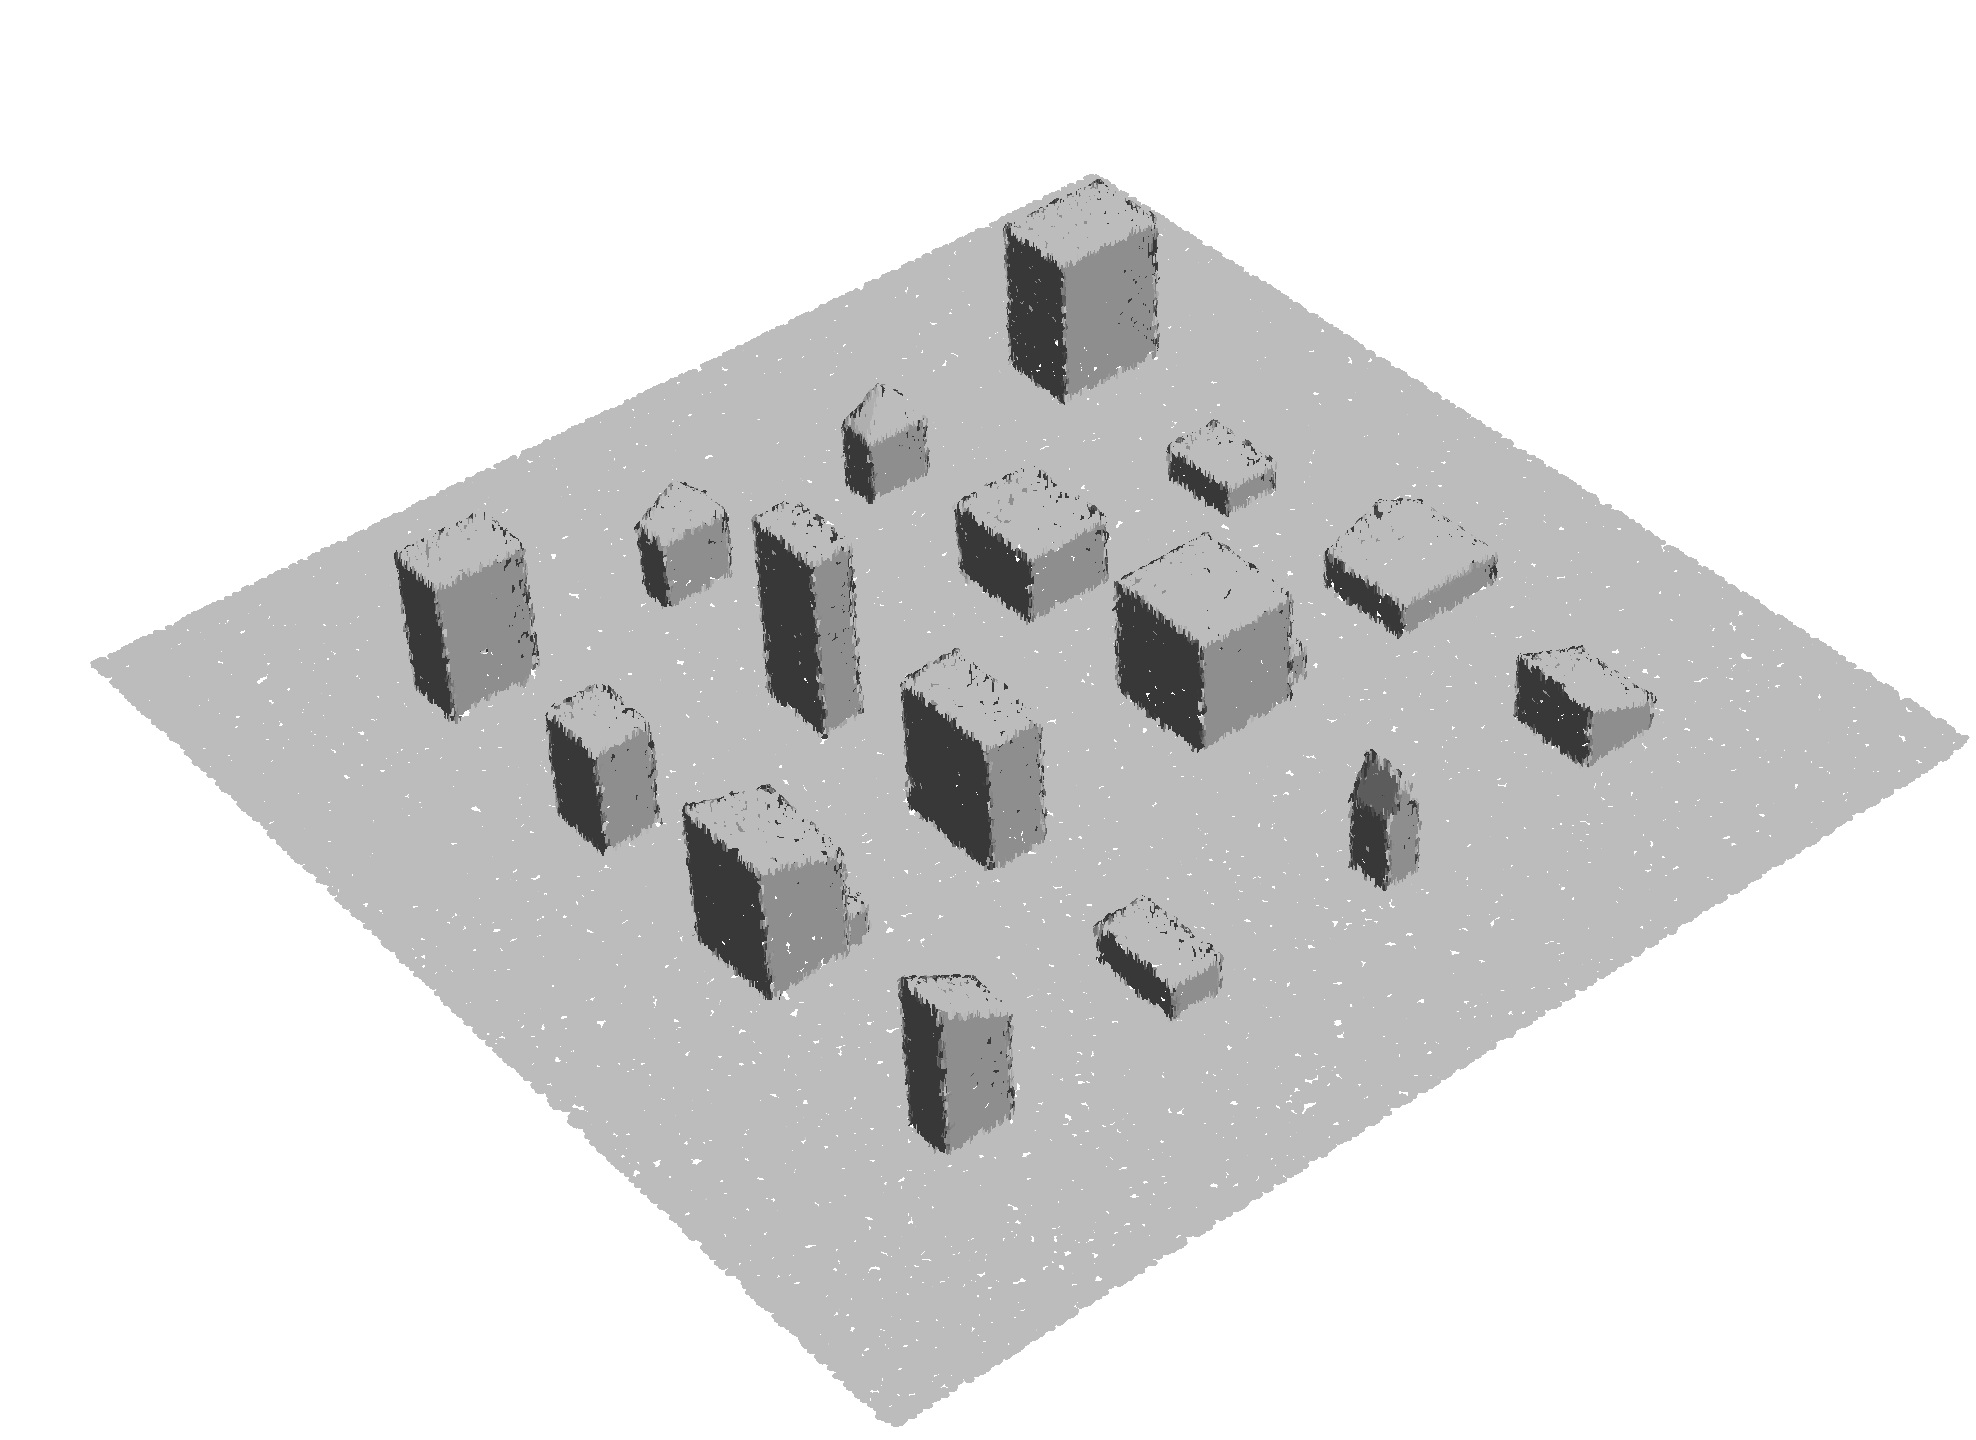
\includegraphics[width=\linewidth]{figs/smat/smat_r3d_surface.png}
		\subcaption{Surface points.}
		\label{fig:smat_r3d_surface}
	\end{subfigure}
	\quad
	\begin{subfigure}[t]{0.45\linewidth}
		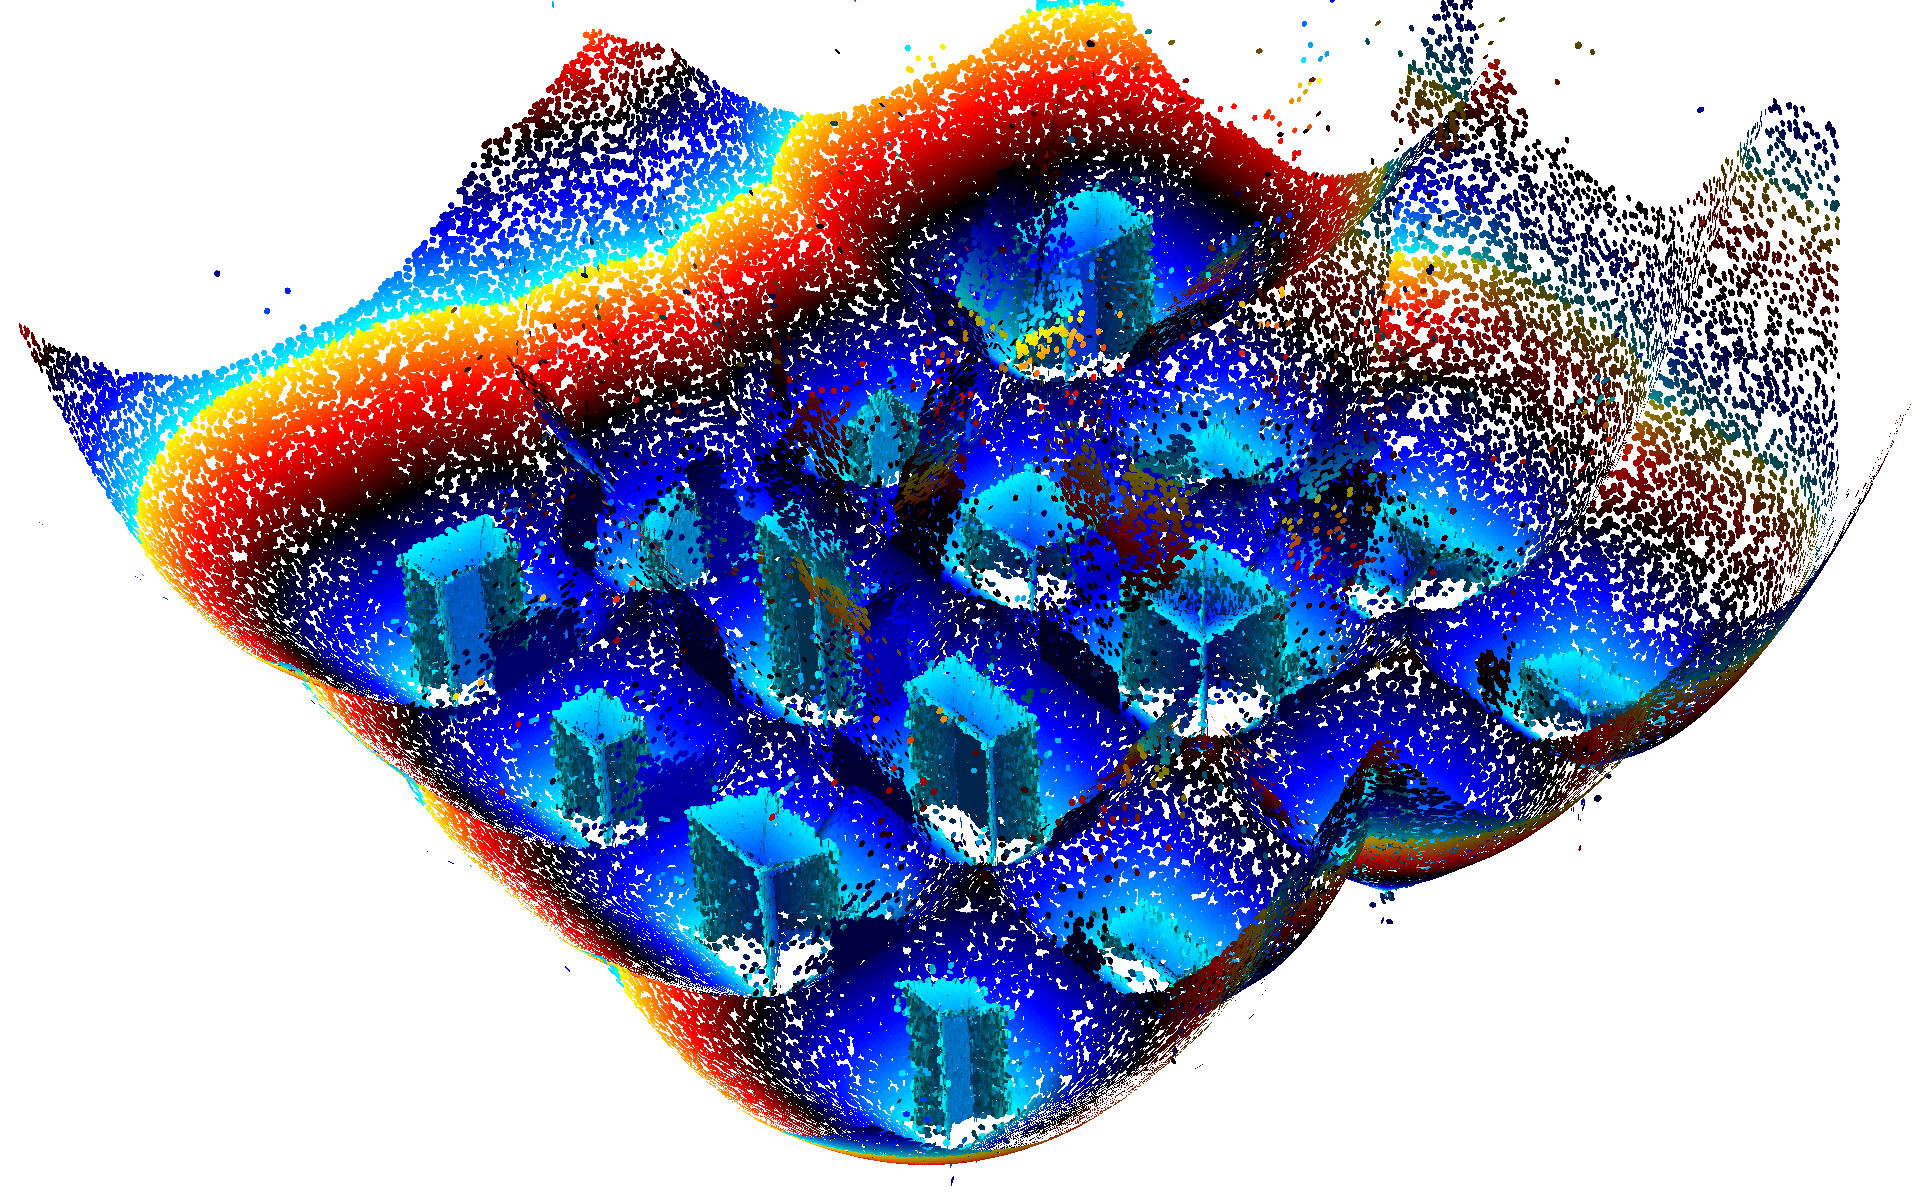
\includegraphics[width=\linewidth]{figs/smat/smat_r3d_mat.png}
		\subcaption{Medial atoms coloured by medial radius using a repeating colourmap.}
		\label{fig:smat_r3d_mat}
	\end{subfigure}
	\quad
	\begin{subfigure}[t]{0.45\linewidth}
		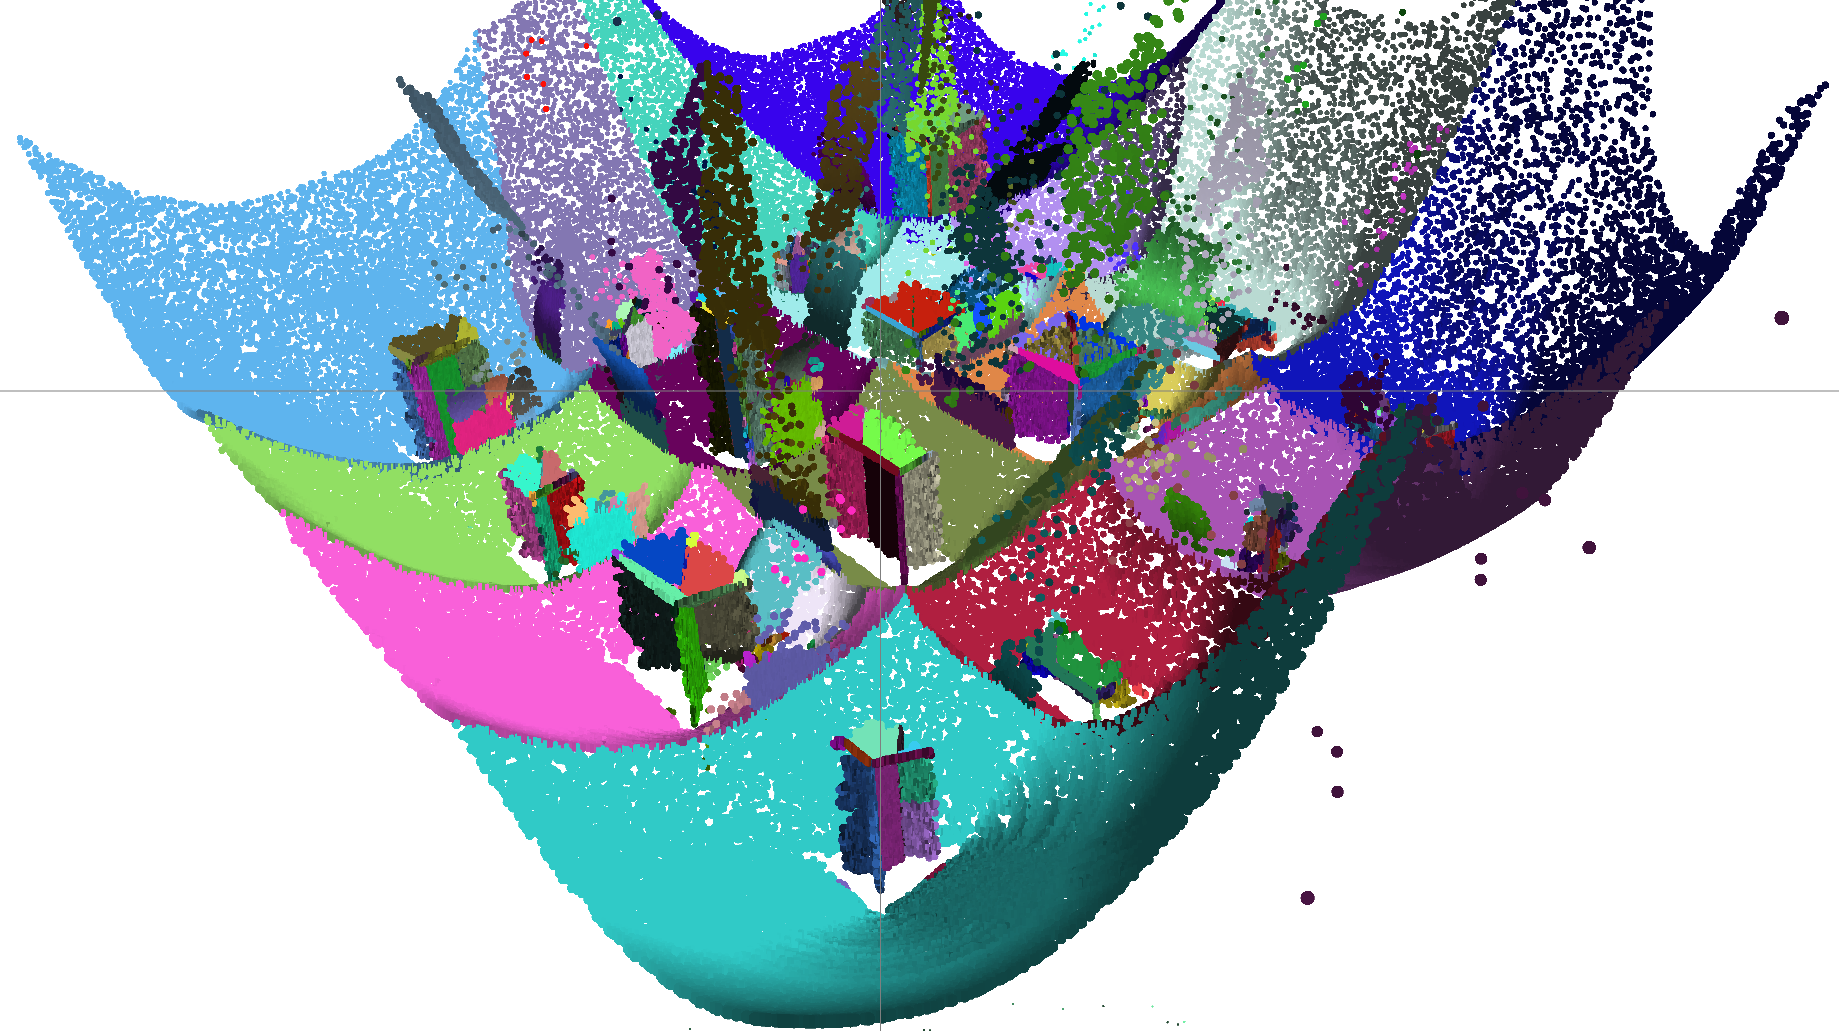
\includegraphics[width=\linewidth]{figs/smat/smat_r3d_thetad_all.png}
		\subcaption{Medial sheet segmentation.}
		\label{fig:smat_r3d_sheets_all}
	\end{subfigure}
	\quad
	\begin{subfigure}[t]{0.45\linewidth}
		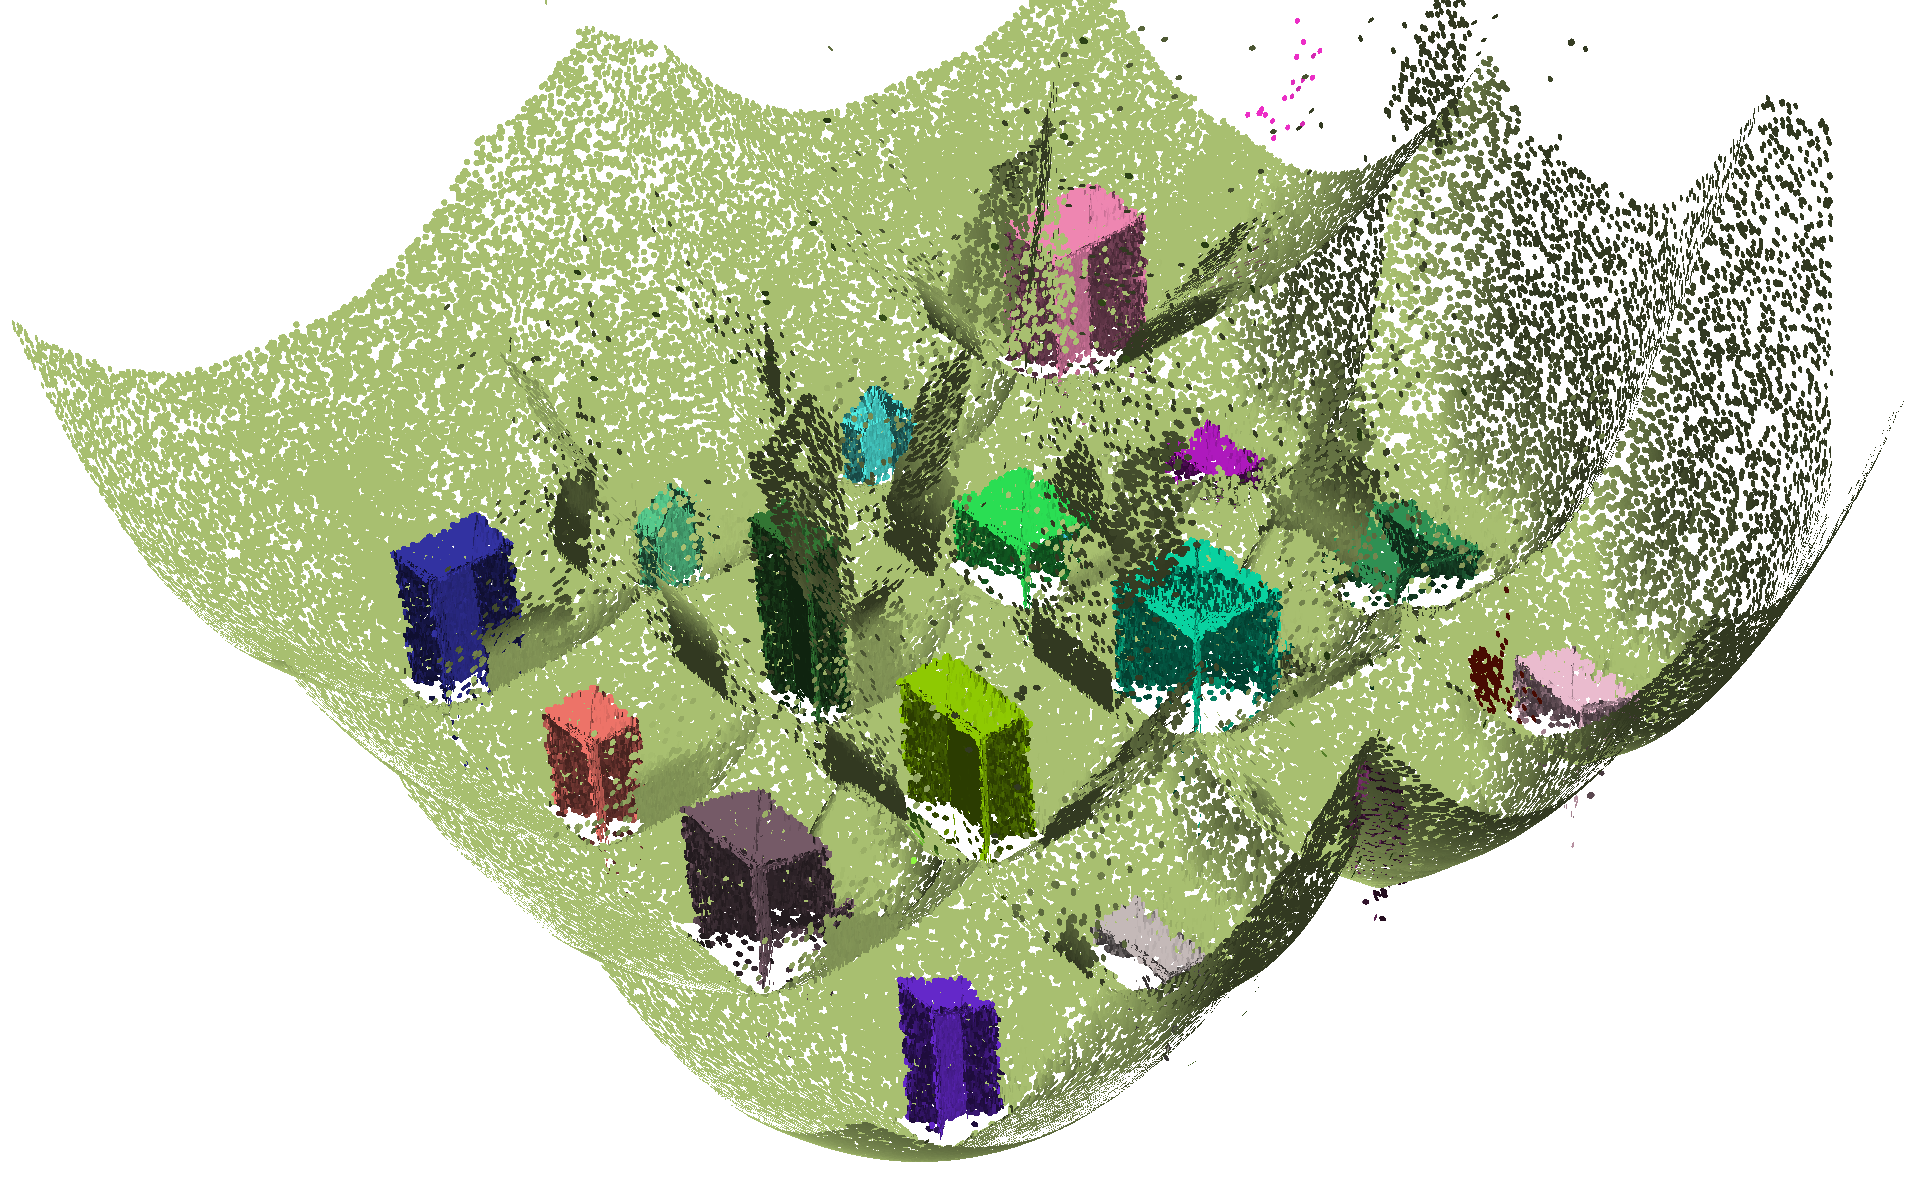
\includegraphics[width=\linewidth]{figs/smat/smat_r3d_ballo_all.png}
		\subcaption{Medial cluster segmentation.}
		\label{fig:smat_r3d_ballo_all}
	\end{subfigure}
	\quad
	\begin{subfigure}[t]{0.45\linewidth}
		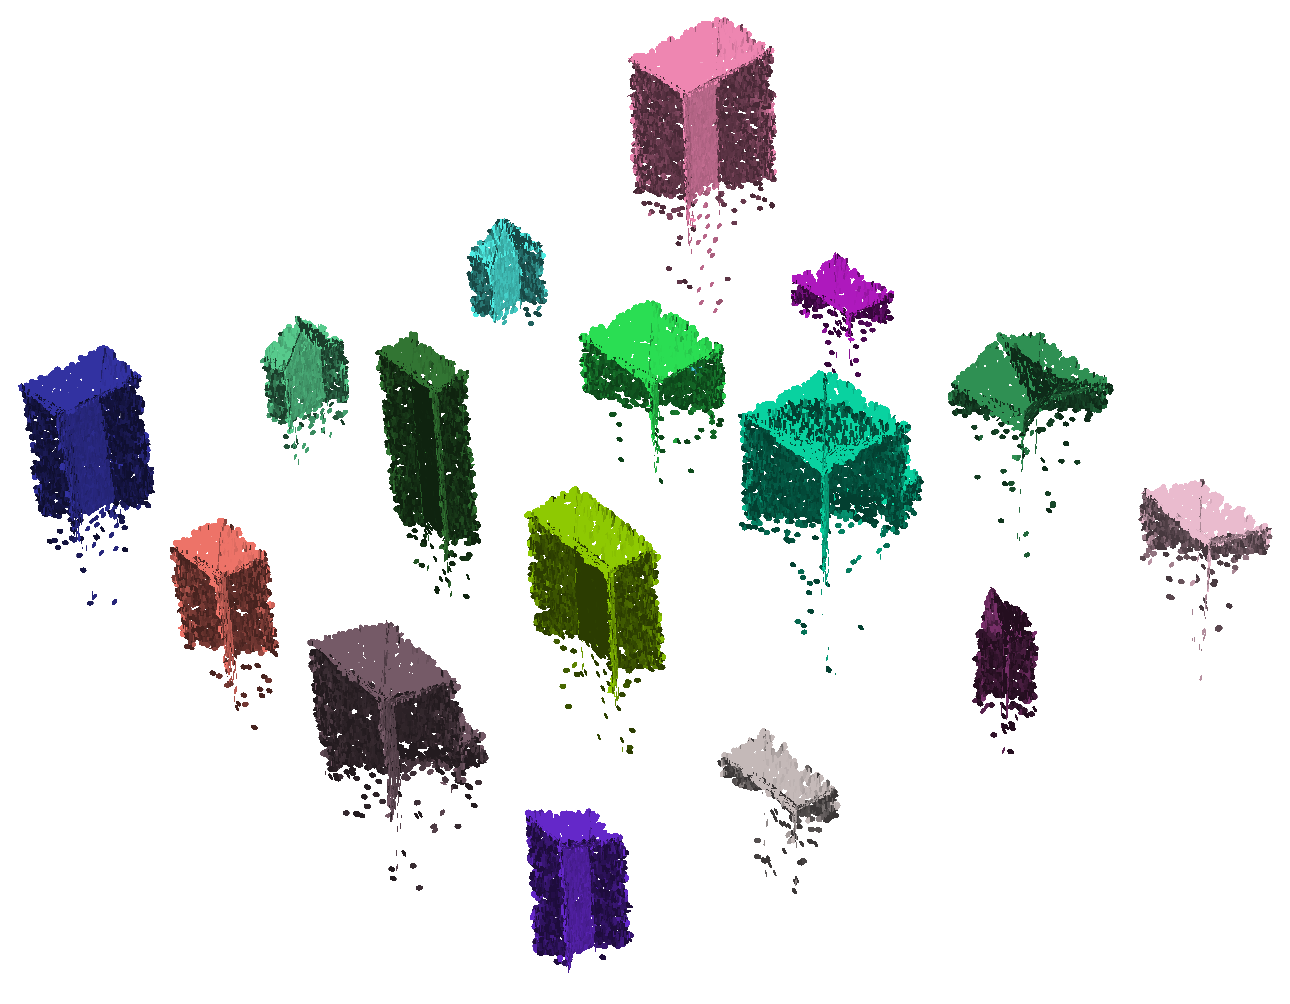
\includegraphics[width=\linewidth]{figs/smat/smat_r3d_mat_int.png}
		\subcaption{Interior medial clusters.}
		\label{fig:smat_r3d_ballo_int}
	\end{subfigure}
	\quad
	\begin{subfigure}[t]{0.45\linewidth}
		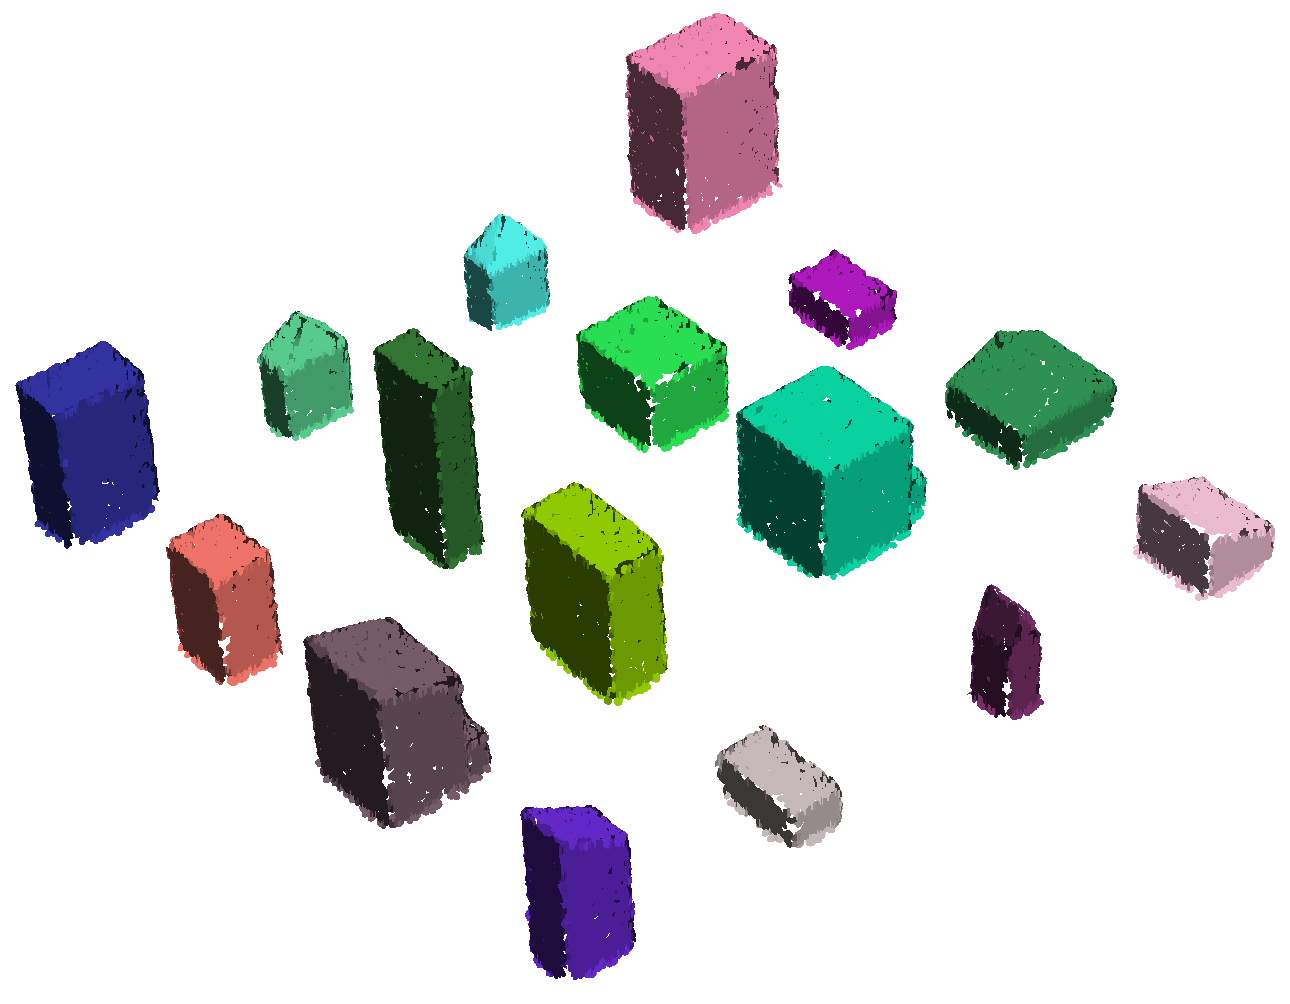
\includegraphics[width=\linewidth]{figs/smat/smat_r3d_surface_int.png}
		\subcaption{Surface points corresponding to interior medial clusters.}
		\label{fig:smat_r3d_surface_int}
	\end{subfigure}
	\caption{Interior MAT part in.}
	\label{fig:smat_r3d_int}
\end{figure}

% \begin{figure}
% 	\centering
% 	\begin{subfigure}{0.45\linewidth}
% 		\centering
% 		\includegraphics[width=\textwidth]{figs/watercourse_crossec_mat.pdf}
% 		\subcaption{Cross section of a watercourse. The 3D skeleton is obtained by reconstructing medial balls that touch the ground surface in two points.}\label{fig:crosssec}
% 	\end{subfigure}
% 	\qquad
% 	\begin{subfigure}{0.45\linewidth}
% 		\centering
% 		\includegraphics[width=\textwidth]{figs/watercourse_3d_mat.pdf}
% 		\subcaption{Perspective view of the 3D skeleton of simple watercourses.}\label{fig:crosssec3d}
% 	\end{subfigure}
% 	\caption[MAT segmentation]{Profile view of 3D skeleton of the terrain}
% 	\label{fig:MAT2D3D}
% \end{figure}

\section{Computing the MAT} 
Computing the MAT from the boundary $\mathcal{B}$ of an object is typically done in two steps. 
During the first step, \ie\ \emph{MAT approximation}, a noisy approximation of the MAT is obtained, and during the second step, \ie\ \emph{pruning}, the noise is removed.

\subsection{MAT approximation}
The MAT can be approximated in various ways, \eg~by using voxels and distance transforms or as a subset of the Voronoi diagram.
In this lesson, however, we will focus on the so-called shrinking-ball algorithm.

\subsubsection{The shrinking-ball algorithm}
The shrinking-ball algorithm works well for robustly approximating the MAT of 3D objects that are represented using boundary points, \ie point clouds.
It is a simple and fast algorithm that can be made robust to noise in the boundary points.
%This means that pruning the MAT after approximation is not necessary with the shrinking-ball algorithm.
The shrinking-ball algorithm takes an \emph{oriented point cloud} as input, \ie\ a point cloud that includes a normal vector for each point. 
It outputs a disjoint set of medial atoms. 

The algorithm is based on the observation that the medial atom corresponding to a boundary point $\mathbf{p}$ must be positioned somewhere on the line $L$ through the normal $\vec{\mathbf{n}}$ of $\mathbf{p}$.
This observation is used to restrict the search space for the medial ball of $\mathbf{p}$ to the line $L$.
As illustrated by Figure~\ref{fig:shrinkballAlgo}, the algorithm begins with a very large candidate ball for $\mathbf{p}$ that is centered on $L$.
\begin{figure}[tbp]
	\begin{subfigure}{0.245\linewidth}
		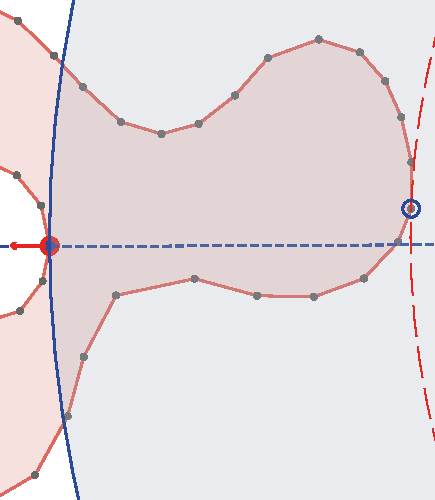
\includegraphics[width=\textwidth]{figs/fullBallShrink_1.pdf}
		\subcaption{Initial ball}
		\label{fig:fullBallShrink_1}
	\end{subfigure}
	\begin{subfigure}{0.245\linewidth}
		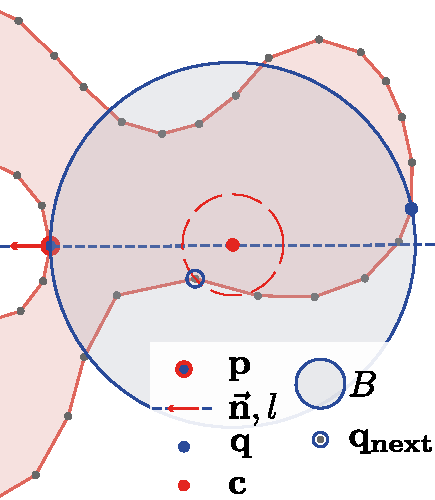
\includegraphics[width=\textwidth]{figs/fullBallShrink_2.pdf}
		\subcaption{Second iteration.}
		\label{fig:fullBallShrink_2}
	\end{subfigure}
	\begin{subfigure}{0.245\linewidth}
		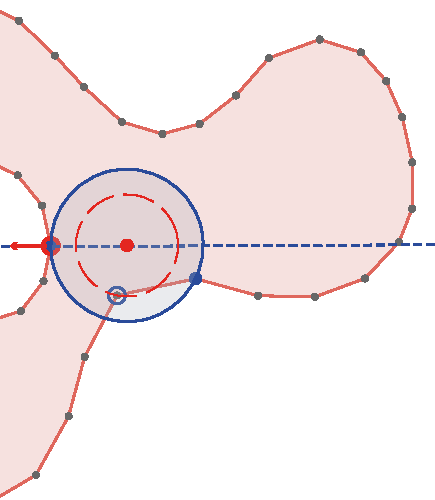
\includegraphics[width=\textwidth]{figs/fullBallShrink_3.pdf}
		\subcaption{Third iteration.}
		\label{fig:fullBallShrink_3}
	\end{subfigure}
	\begin{subfigure}{0.245\linewidth}
		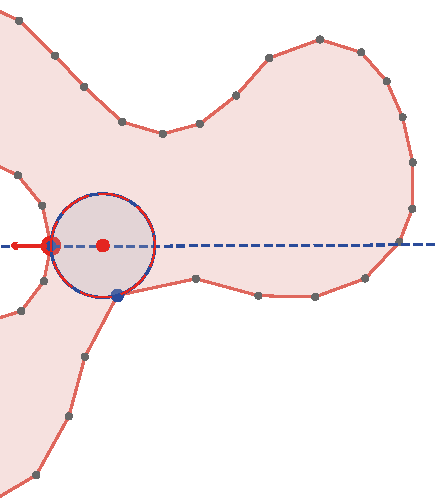
\includegraphics[width=\textwidth]{figs/fullBallShrink_4.pdf}
		\subcaption{Fourth iteration.}
		\label{fig:fullBallShrink_4}
	\end{subfigure}
	\caption{Ball shrinking iterations with the shrinking-ball algorithm. The final iteration yields a \emph{medial} ball. A legend is given in \subref{fig:fullBallShrink_2}.}
	\label{fig:shrinkballAlgo}
\end{figure}
At each consecutive iteration, a new candidate ball is constructed that is smaller than the previous one and closer to the final \emph{medial} ball.
Every ball is constructed so that it touches $\mathbf{p}$ and is centred on $L$.
Only the candidate feature point $\mathbf{q}$ changes with each iteration.
A new $\mathbf{q}$, denoted $\mathbf{q_{next}}$, is found by selecting the closest point from the centre $\mathbf{c}$ of the current ball.
Using $\mathbf{p}, \vec{\mathbf{n}}, \mathbf{q_{next}}$ we can compute the centre of the next ball $\mathbf{c_{next}}$, at which point we move on to the next iteration.
The algorithm terminates when an empty ball is found, which is the case when the radius no longer shrinks.
Algorithm~\ref{alg:shrinkBall} gives the pseudo-code for the shrinking-ball algorithm.
\begin{algorithm}[tb]
	\SetKwInOut{Input}{Input}
	\SetKwInOut{Output}{Output}
	\DontPrintSemicolon\Input{
		a KD-tree of the surface point cloud $T$,\\ 
		a surface point $\mathbf{p}$\\ 
		it's normal vector $\vec{\mathbf{n}}$, and\\
		the initial ball radius $r_{init}$}
	\Output{the medial ball centre $\mathbf{c}$,\\the medial ball radius $r$}
	$r \leftarrow r_{init}$ \\
	$\mathbf{c} \leftarrow$ the centre of the ball that touches $\mathbf{p}$ is centered on $\vec{\mathbf{n}}$ with a radius $r$ \\
	\Repeat{a \textbf{break} statement is executed} {
		$q_{next} \leftarrow$ the nearest point to $\mathbf{c}$, obtained quickly using $T$ \\
		$r_{next} \leftarrow$ radius of the next ball that touches $\mathbf{p}$ and $\mathbf{q_{next}}$ and is centred on $\vec{\mathbf{n}}$ \\
		$\mathbf{c_{next}} \leftarrow$ centre of the next ball, can be computed with $\mathbf{p}, \vec{\mathbf{n}}$, and $r_{next}$ \\
		\If{$r_{next} = r$} {
			\textbf{break}
		}
		$\mathbf{c} \leftarrow \mathbf{c_{next}}$ \\
		$r \leftarrow r_{next}$
	}
	\caption{The shrinking-ball algorithm.}
	\label{alg:shrinkBall}
\end{algorithm}

The algorithm is run for each point in the input point cloud. 
If the normal vectors point away from the interior, the interior MAT is computed.
And by flipping the orientation of the normal vector, the exterior MAT can also be computed.
If normals are not available for a point cloud, these can be estimated using local plane fitting, \ie\ by fitting a plane to the $k$ nearest neighbours of each boundary point. 
The vector perpendicular to that plane then becomes the estimated normal vector.
A KD-tree is typically used to speed up the nearest neighbour searches, both for normal estimation and the shrinking-ball algorithm.
Figure~\ref{fig:ca_ridge} gives an example result of the shrinking-ball algorithm for a terrain point cloud. 
Observe how the MAT describes the valleys (exterior MAT) and ridges (interior MAT) in the terrain with its skeletal structure.
\begin{figure}
	\centering
	\begin{subfigure}{0.310\linewidth}
		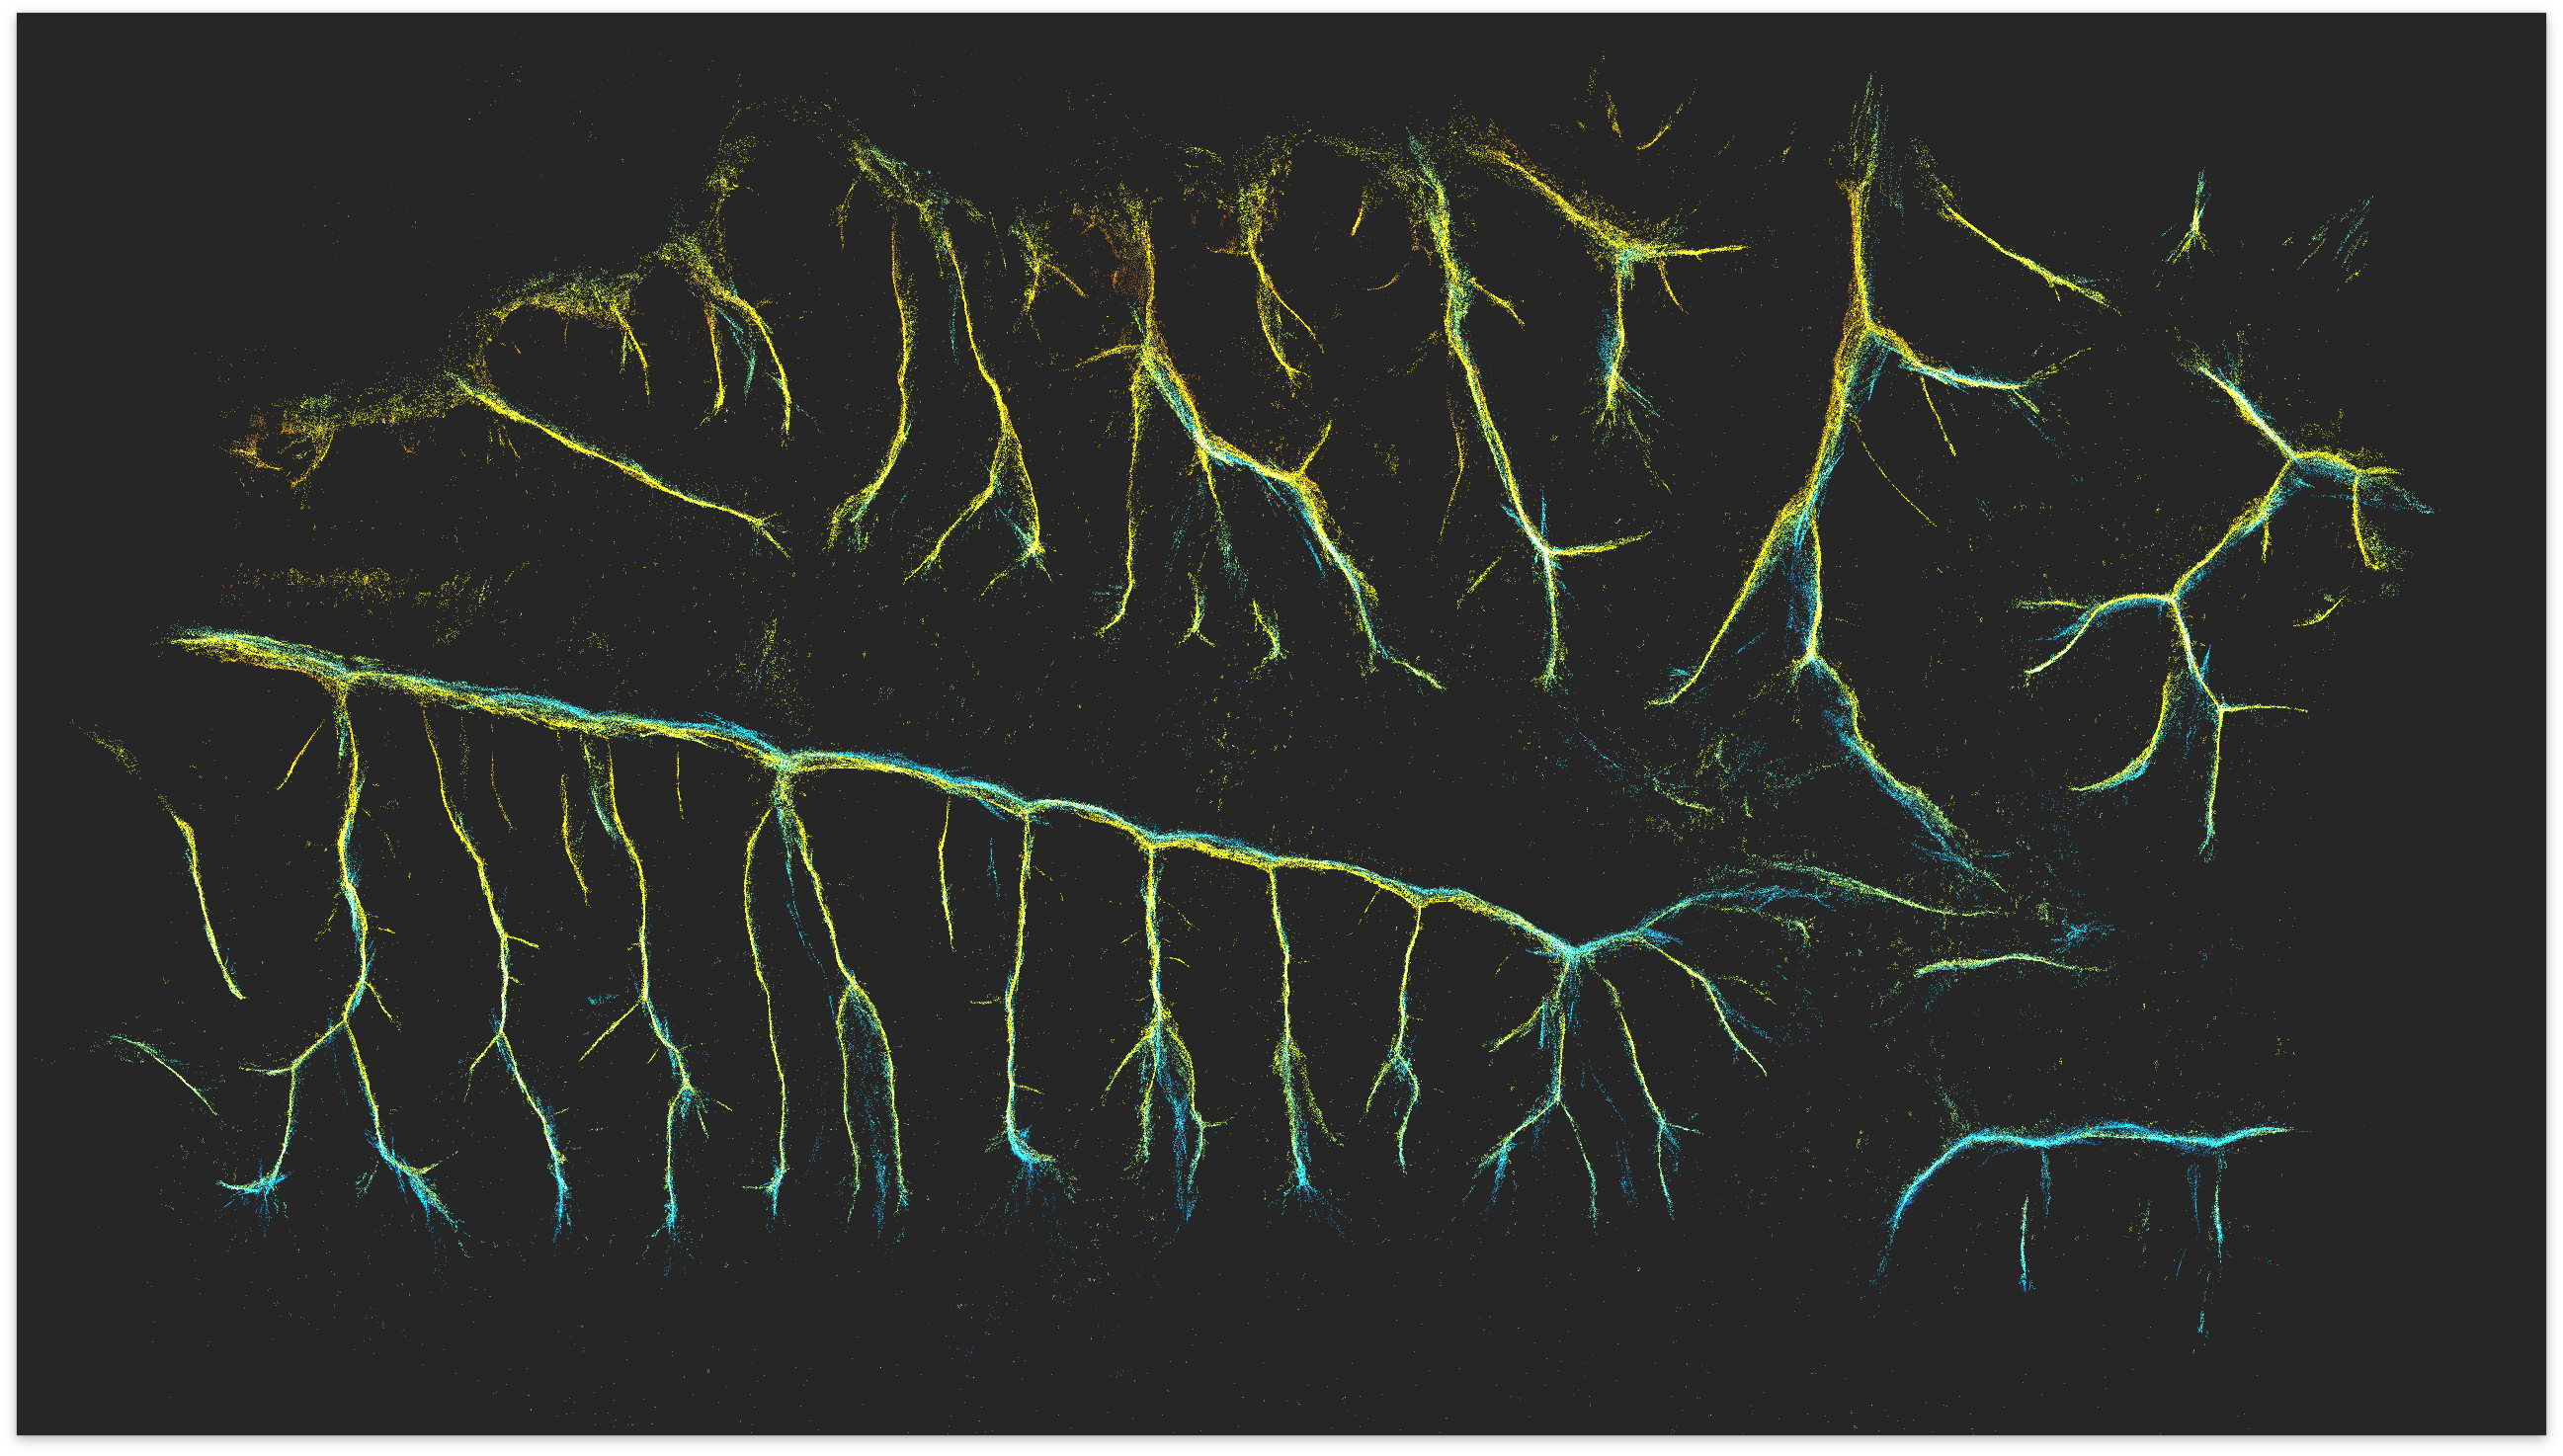
\includegraphics[angle=90,width=\linewidth]{figs/iMAT.png}
		\caption{Interior MAT.}
		\label{fig:ca_ridge:imat}
	\end{subfigure}
	\quad
	\begin{subfigure}{0.310\linewidth}
		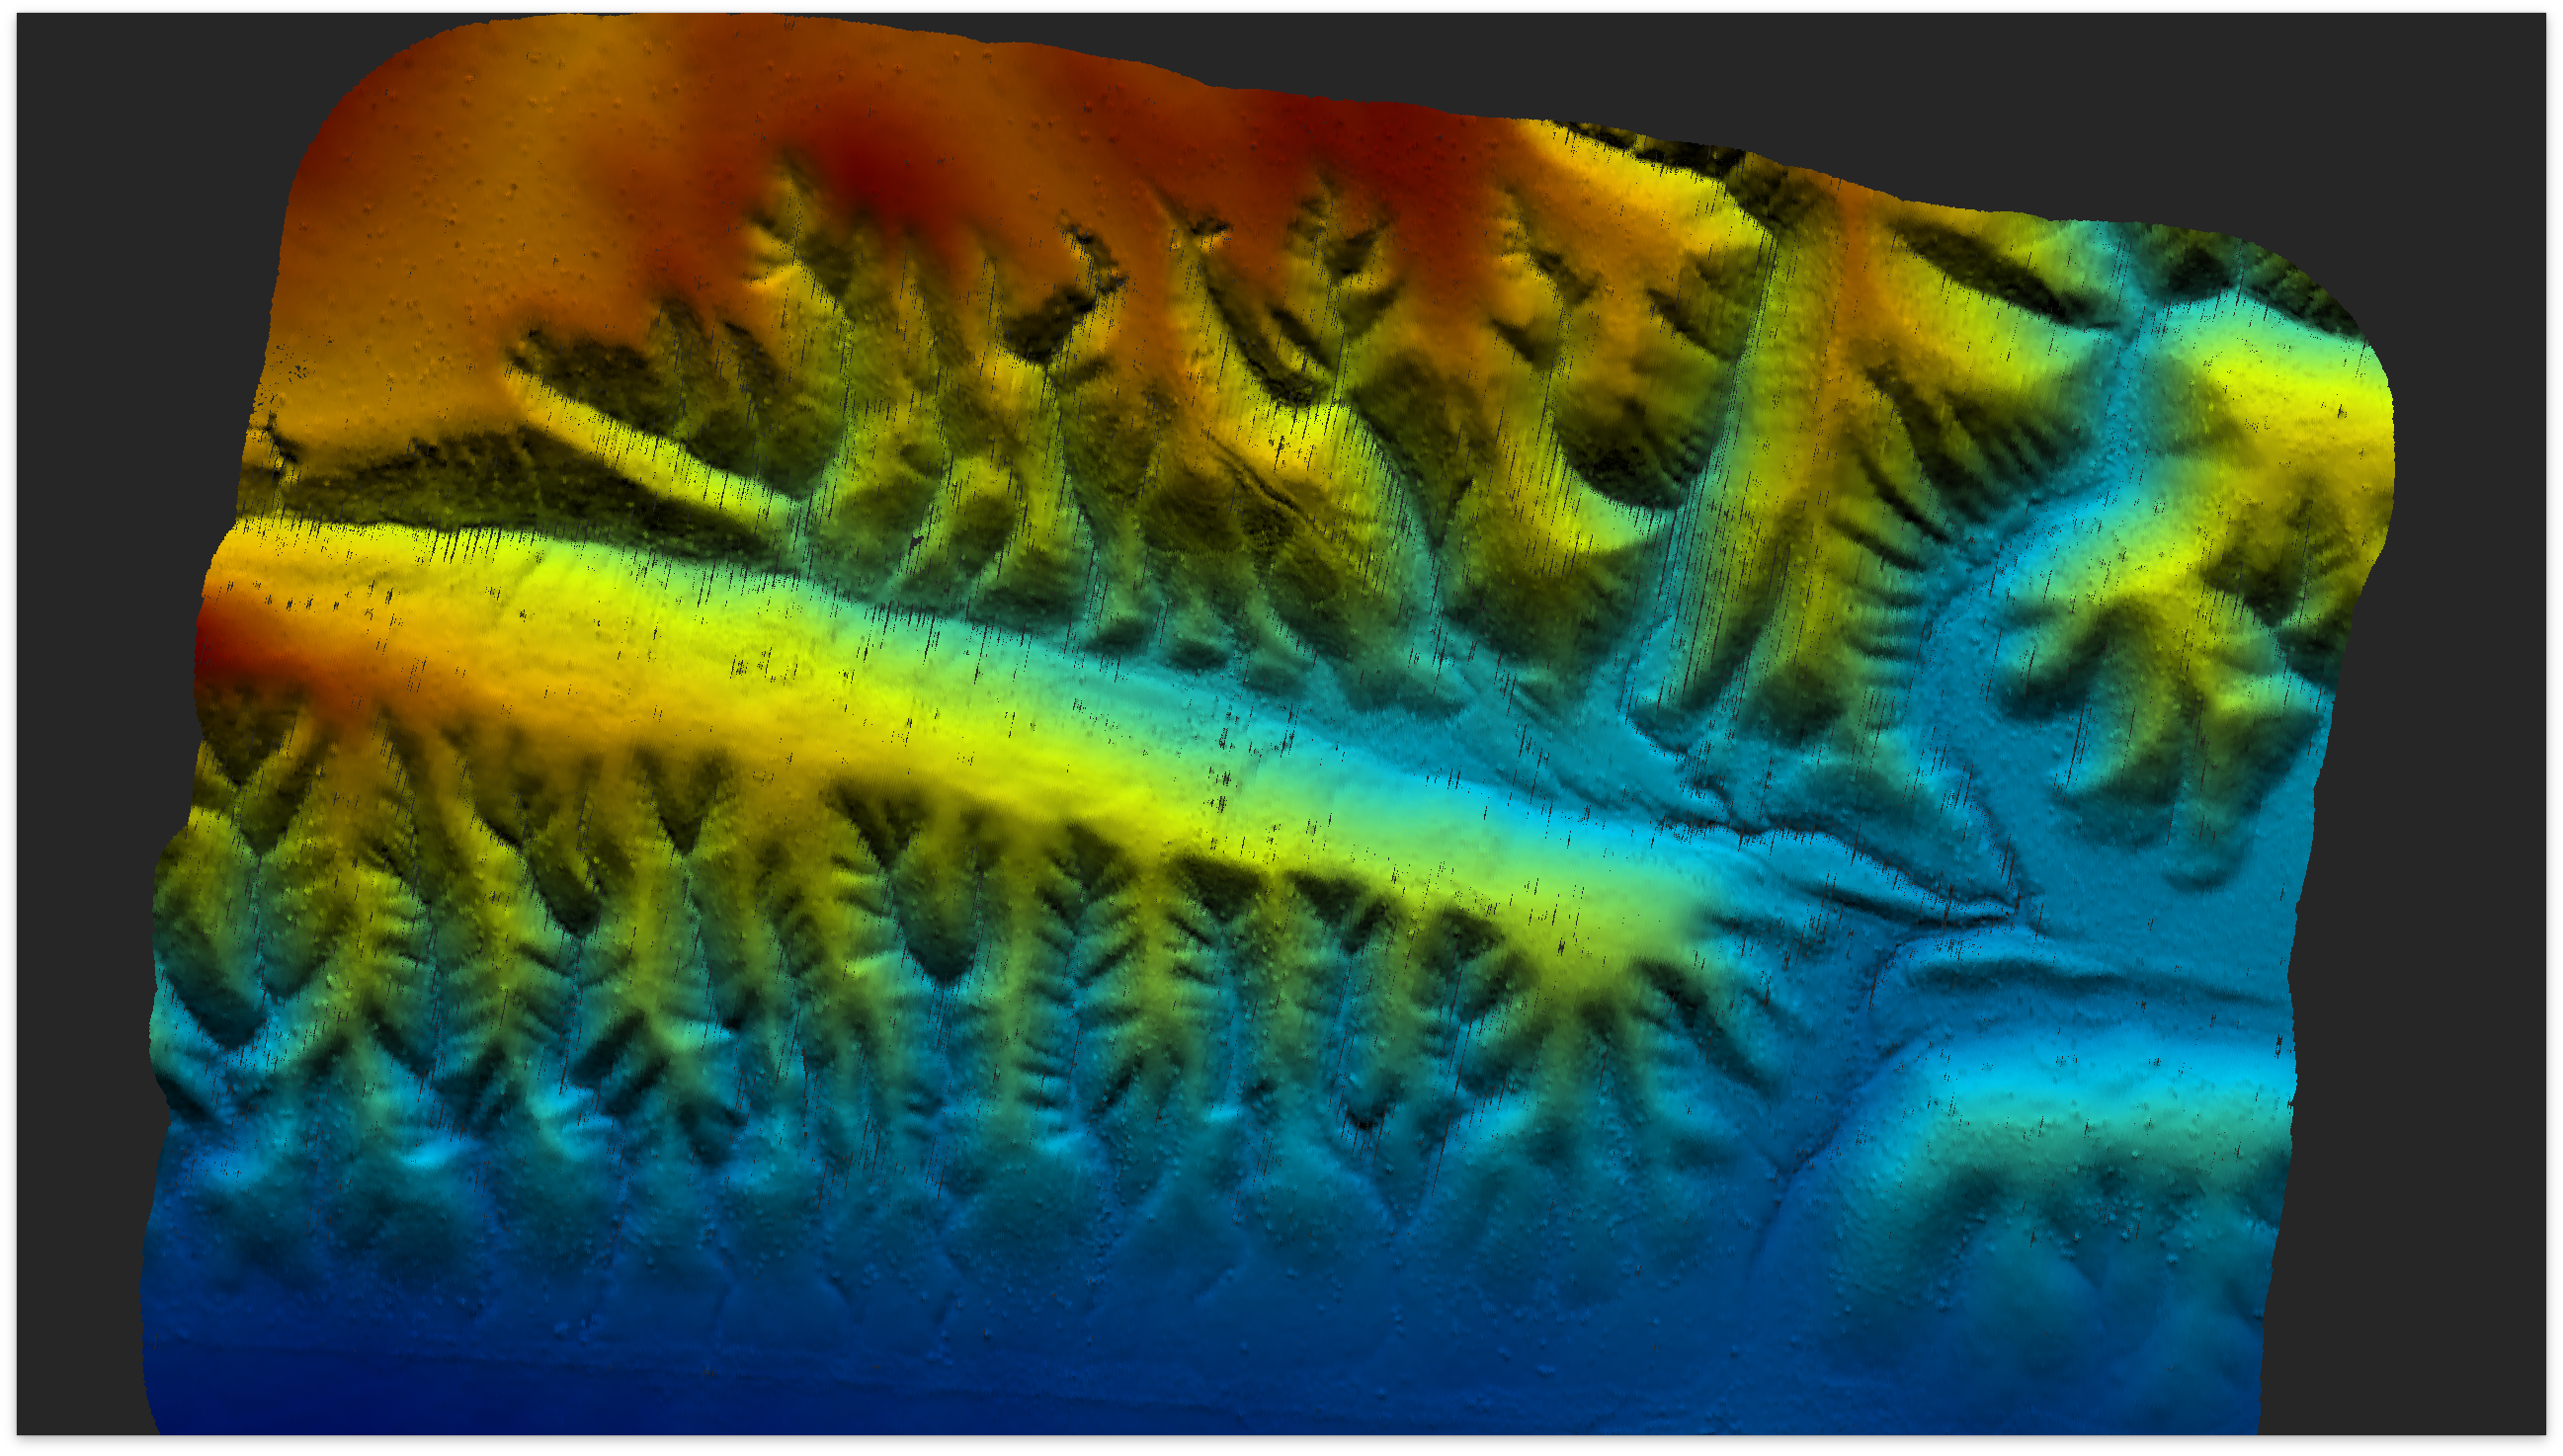
\includegraphics[angle=90,width=\linewidth]{figs/terrain.png}
		\caption{Terrain points}
		\label{fig:ca_ridge:terrain}
	\end{subfigure}
	\quad
	\begin{subfigure}{0.310\linewidth}
		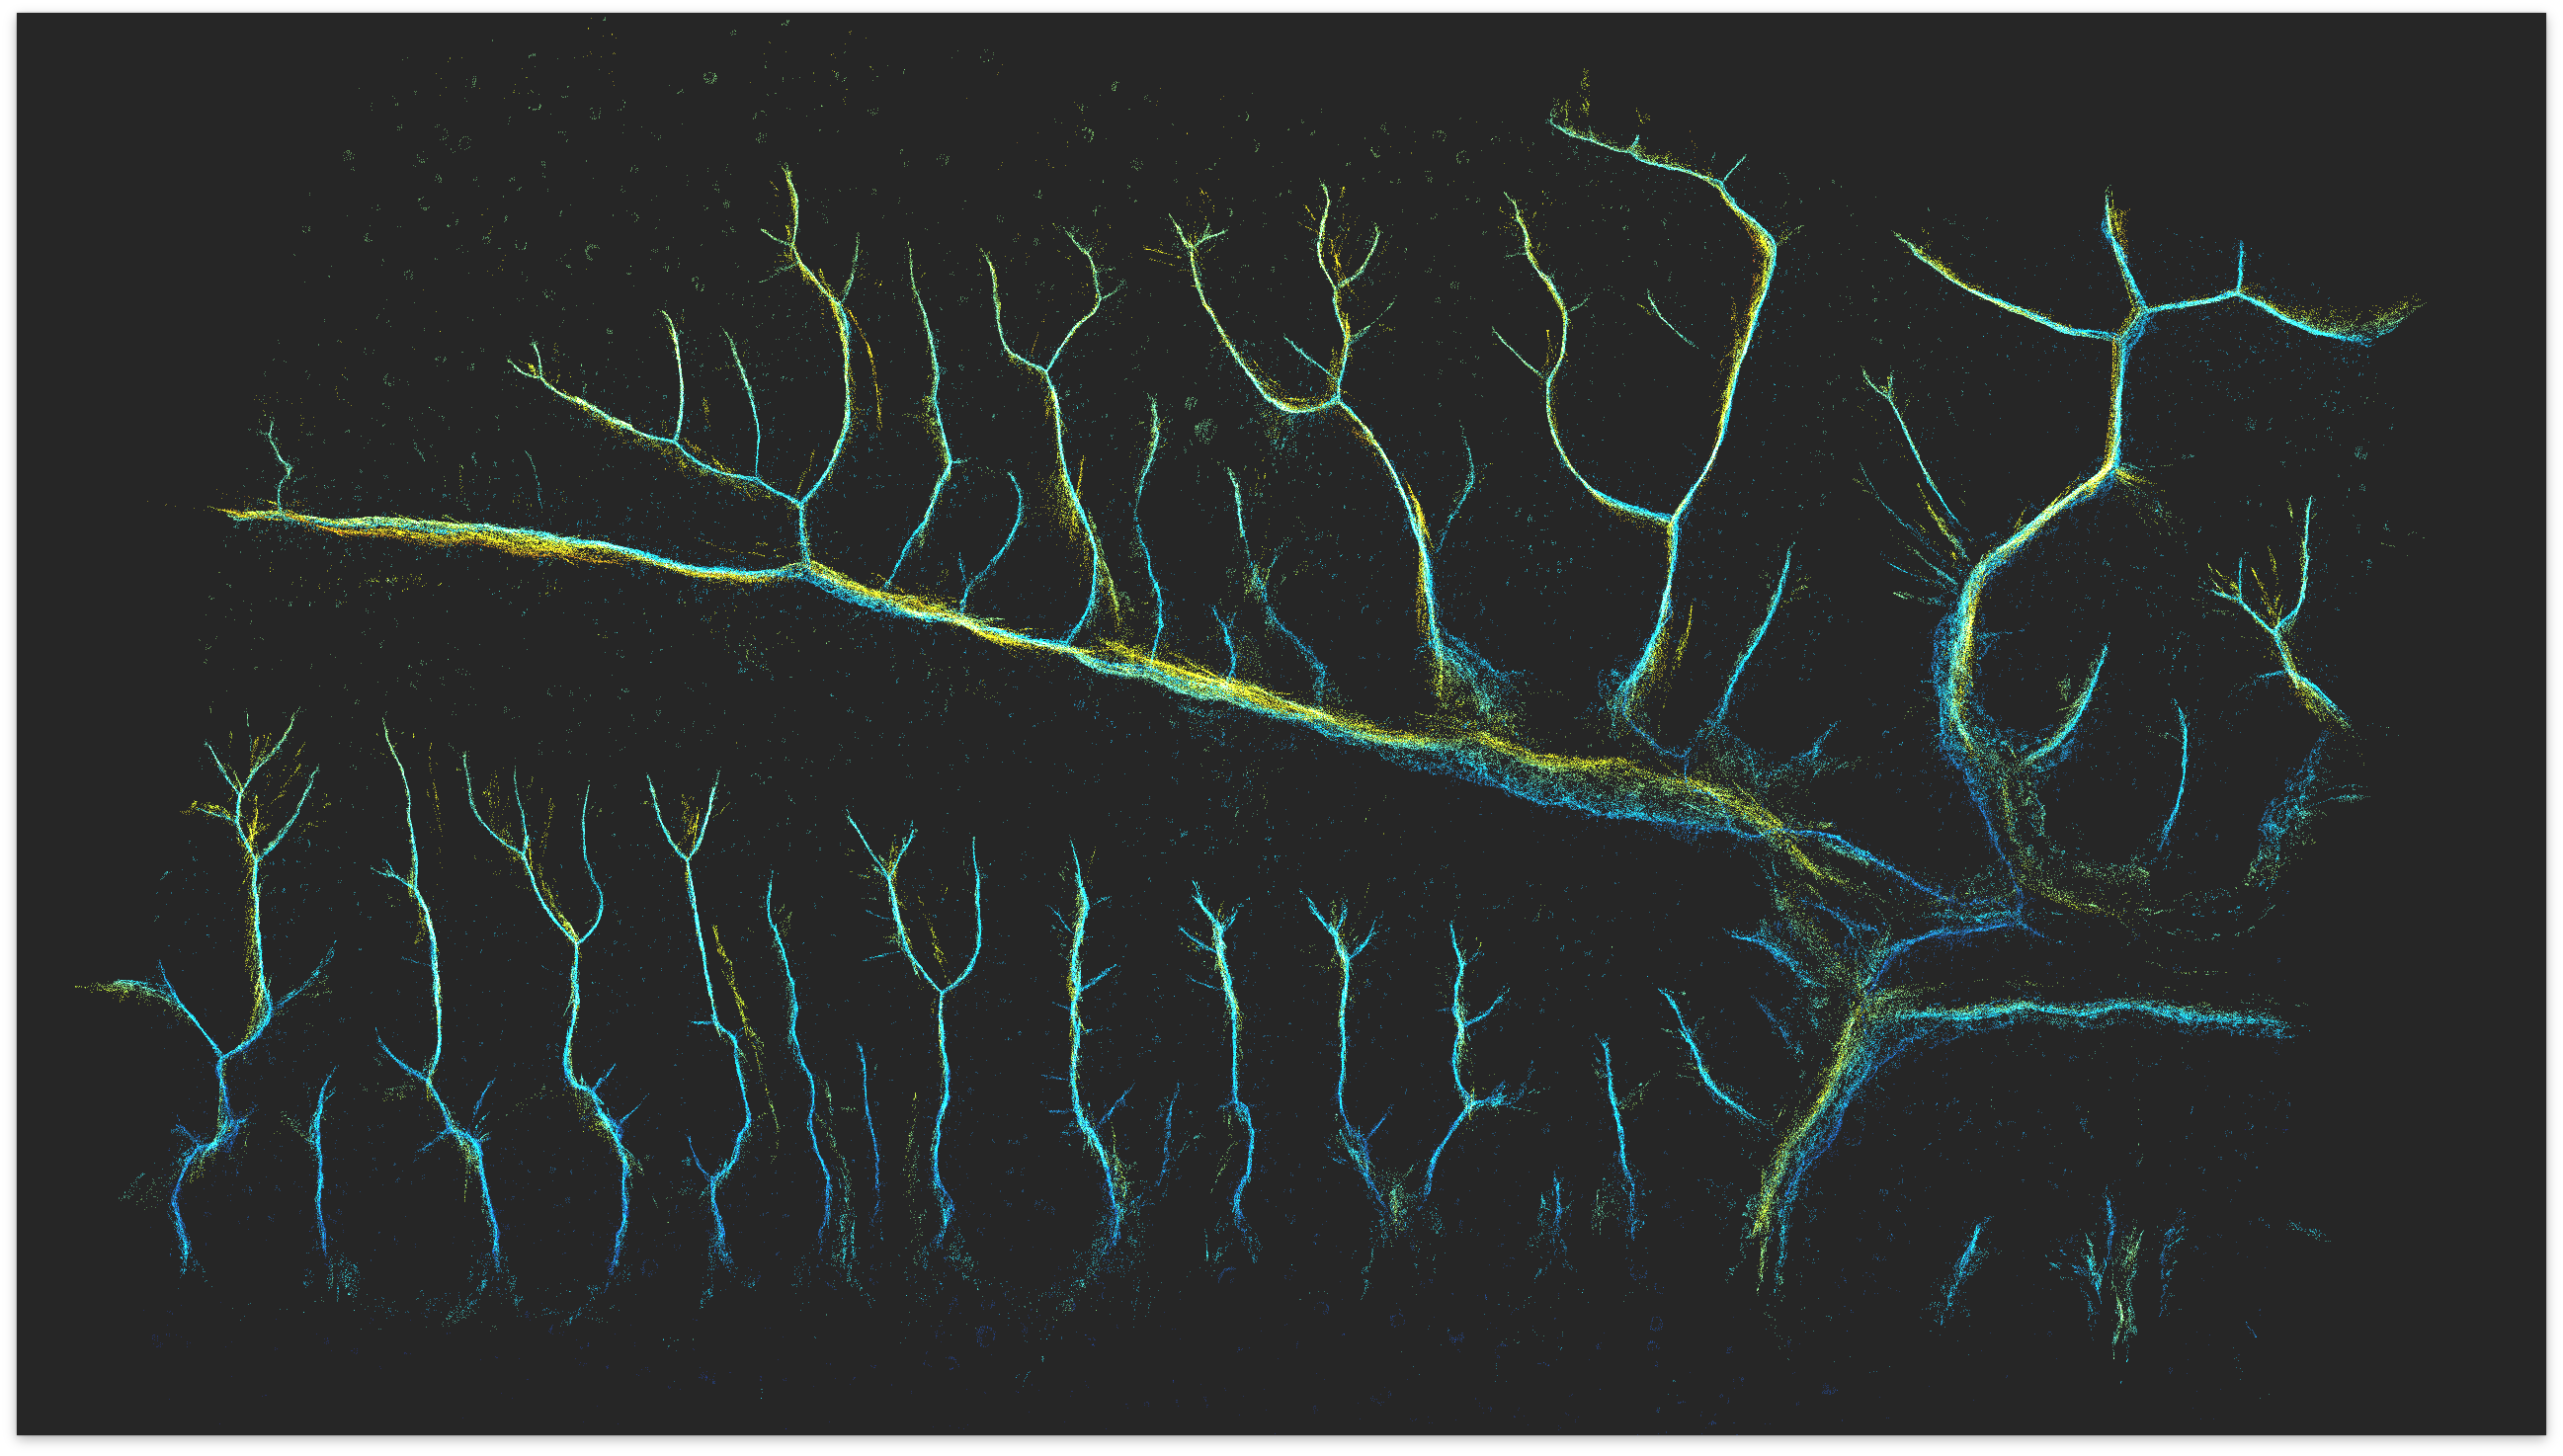
\includegraphics[angle=90,width=\linewidth]{figs/oMAT.png}
		\caption{Exterior MAT}
		\label{fig:ca_ridge:omat}
	\end{subfigure}
	\caption{MAT approximation (a,c) of a lidar terrain point cloud (b) obtained with the shrinking-ball algorithm. Top view.}
	\label{fig:ca_ridge}
\end{figure}

Notice that the shrinking ball algorithm subdivides the output only in an interior and exterior part based on the point normals in the input. 
It is possible to further segment the MAT into for example medial sheets and medial clusters.
This can be achieved for example with a region-growing segmentation algorithm that uses properties of the medial geometry (\eg\ the medial bisector). 
Figures~\ref{fig:smat_r3d_sheets_all} and \ref{fig:smat_r3d_ballo_all} show the result of such a segmentation.

% The main limitation of the shrinking-ball algorithm is that it outputs only an unstructured set of medial atoms, \ie\ there is no distinction between its different medial sheets.% and also the surface of the sheets is not explicitly reconstructed.
% This can be solved by using the medial geometry of the medial atoms.
% Several properties of the medial geometry are locally similar within the same medial sheet.
% With a region-growing algorithm this similarity can be exploited to segment the unstructured medial atoms into medial sheets.
% Especially the medial bisector is useful, \ie\ it is tangential to the medial sheet and it always points in the direction of decreasing radius in a sheet, usually away from junction curves.
% It is thus not only similar within one sheet, but also dissimilar for the different sheets that meet at a junction curve.
% As a result there is little chance that a sheet segment grows into another sheet through a junction curve, leading to well separated sheets (see Figure~\ref{fig:MATmeth}).
% Region-growing can also be used to segment the MAT of a DTM in its different disjoint medial clusters.
% In this case the region-growing condition may be based on a measure for the amount of overlap between nearby medial balls.
% Because, nearby medial balls within one medial cluster are likely to overlap, whereas medial balls between different clusters are not.

\subsection{Pruning}
Pruning is the process of retracting or removing unimportant branches from the MAT.
It is often necessary because the MAT is unstable, \ie\ it is extremely sensitive to small bumps in $\mathcal{B}$.
As illustrated in Figures~\ref{fig:mat-instability} and \ref{fig:imaimp:a}, tiny deviations in $\mathcal{B}$ can lead to big spurious branches in the structure of the MAT.
\begin{figure}
	\centering
	\begin{subfigure}{0.425\linewidth}
		\centering
		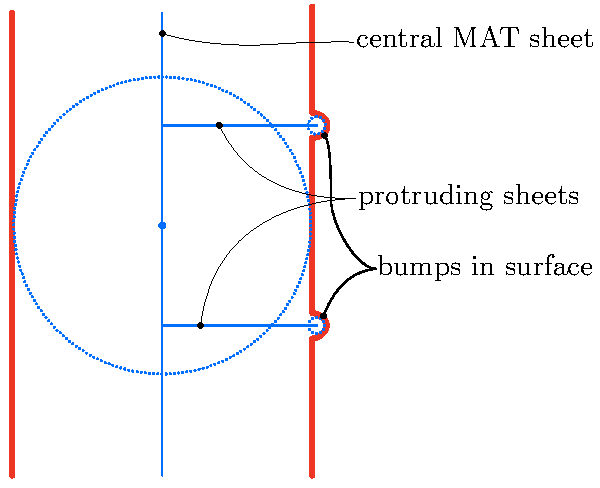
\includegraphics[width=\textwidth]{figs/protrudingSheets.pdf}
		\subcaption{Small bumps in the boundary can cause big spurious branches to appear. Object boundary drawn in red, MAT in blue.}\label{fig:mat-bumps}
	\end{subfigure}
	\qquad
	\begin{subfigure}{0.50\linewidth}
		\centering
		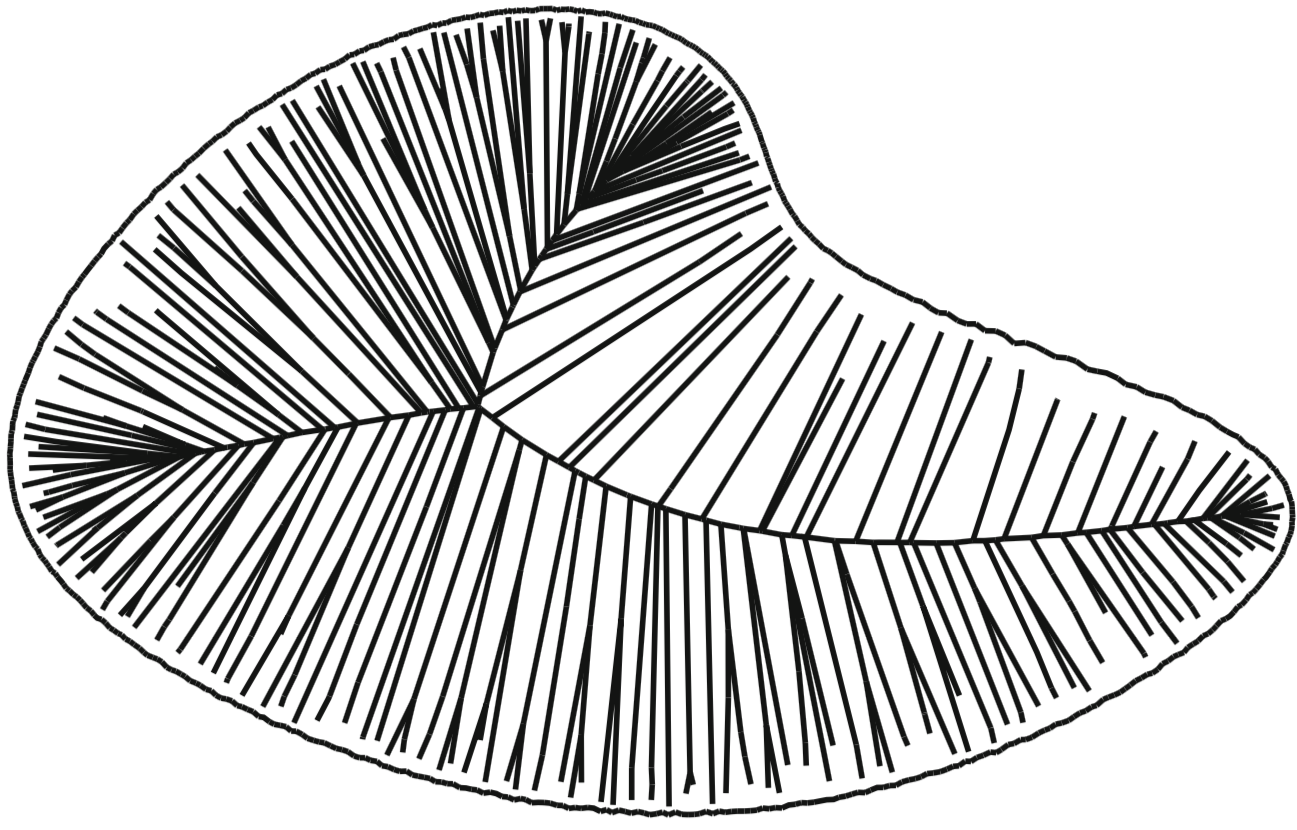
\includegraphics[width=\textwidth]{figs/spurious_branches.png}
		\subcaption{Spurious branches can appear in the MAT due to a small amount of noise in the boundary.}
		\label{fig:sb_noise}
	\end{subfigure}
	\caption{Instability of the MAT.}
	\label{fig:mat-instability}
\end{figure}
This is especially problematic when $\mathcal{B}$ has some noise as is the case with the typical DTM.
The resulting MAT can become so distorted by the spurious branches that it becomes hard to distinguish its main medial structure.
The main aim of pruning is to remove these spurious branches.

Most pruning methods are based on properties of the medial geometry. 
Based on these properties, an importance measure for each medial atom is defined, which is then used as a threshold to filter medial atoms. 
The resulting (pruned) MAT is usually a subset of the original MAT. 
Some methods preserve topology, others do not or do so only up to a certain level. 
The main challenge is often selecting the optimal threshold value---a compromise between removing noisy MAT parts and not removing fine detail, \ie\ often the endpoints of good MAT branches are also affected by pruning.
Examples of importance measures for pruning are the separation angle $\theta$ (recall this is the angle between the spoke vectors) and the separation distance $\lambda$, \ie the distance between the two feature points of a medial atom. 
These values are typically low for noisy parts of the MAT.
Figure~\ref{fig:imaimp} gives an example of pruning with the separation distance.
\begin{figure}
	\centering
	\begin{subfigure}{0.4\linewidth}
		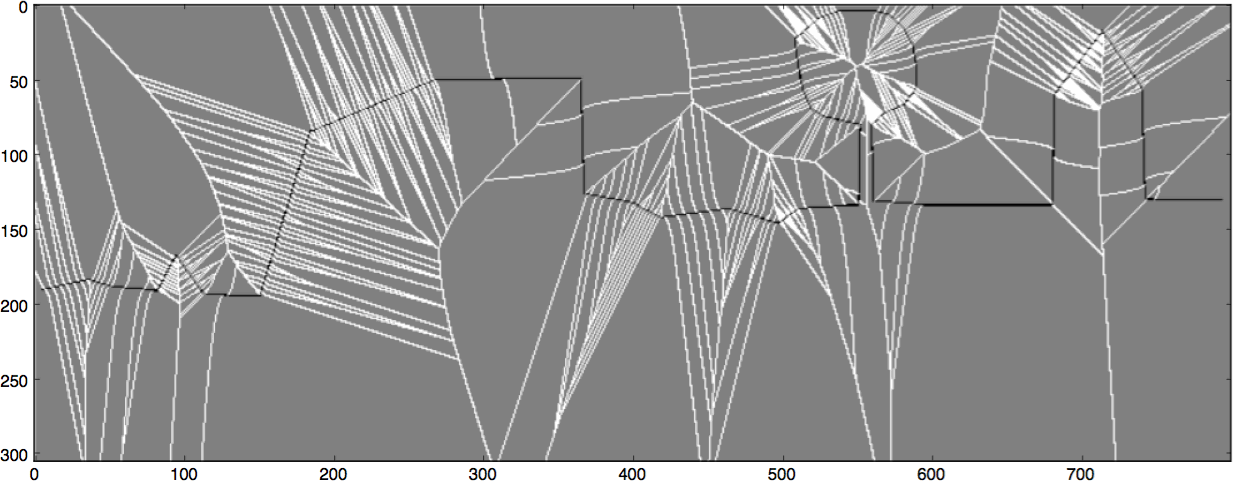
\includegraphics[width=\linewidth]{figs/rasterimpl/simple_dtm-gamma1_earthskel_.png}
		\caption{MAT without pruning ($\lambda=0$)}
		\label{fig:imaimp:a}
	\end{subfigure}
	\quad
	\begin{subfigure}{0.4\linewidth}
		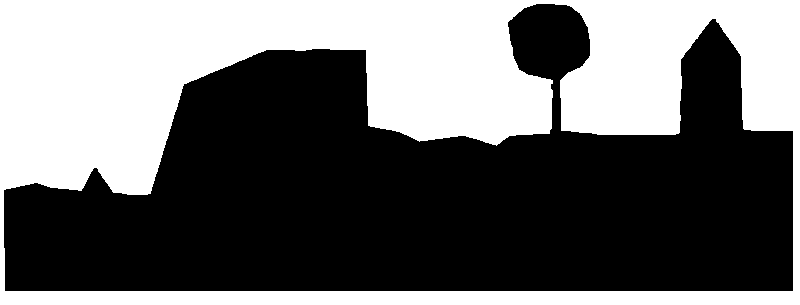
\includegraphics[width=\linewidth]{figs/rasterimpl/simple_dtm-gamma1_earthskel.png}
		\caption{Reconstructed object for $\lambda=0$.}
		\label{fig:imaimp:b}
	\end{subfigure}
	
	\begin{subfigure}{0.4\linewidth}
		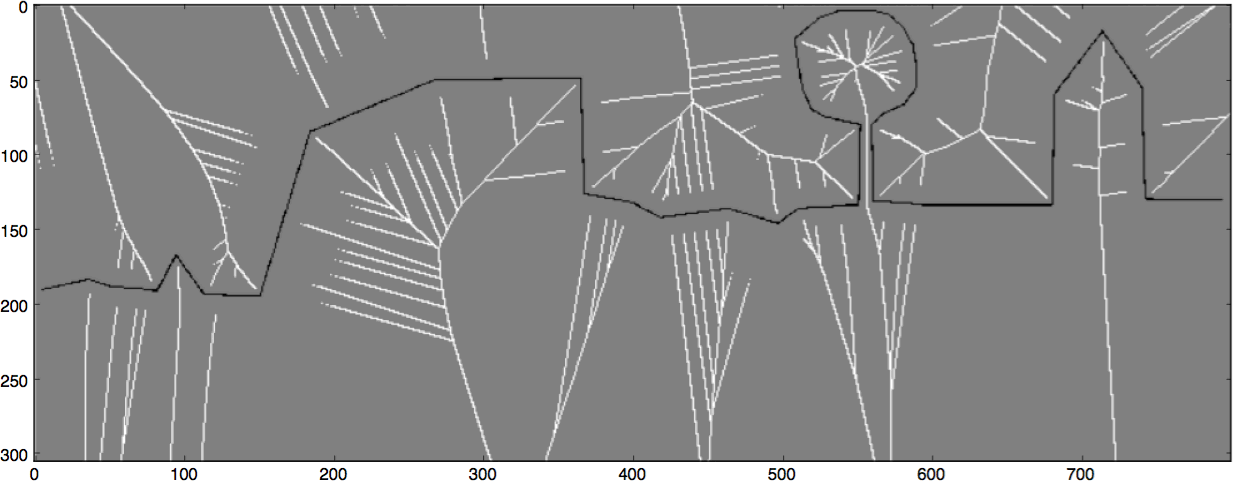
\includegraphics[width=\linewidth]{figs/rasterimpl/simple_dtm-gamma6_earthskel_.png}
		\caption{MAT with medium pruning ($\lambda=6$)}
		\label{fig:imaimp:c}
	\end{subfigure}
	\quad
	\begin{subfigure}{0.4\linewidth}
		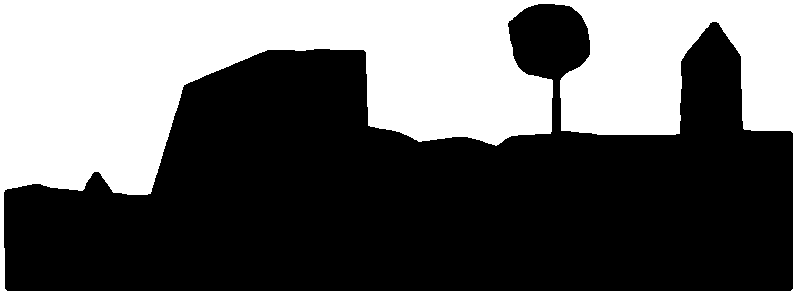
\includegraphics[width=\linewidth]{figs/rasterimpl/simple_dtm-gamma6_earthskel.png}
		\caption{Reconstructed object for $\lambda=6$. Despite the pruned MAT, the corresponding boundary remains almost unchanged.}
		\label{fig:imaimp:d}
	\end{subfigure}
	
	\begin{subfigure}{0.4\linewidth}
		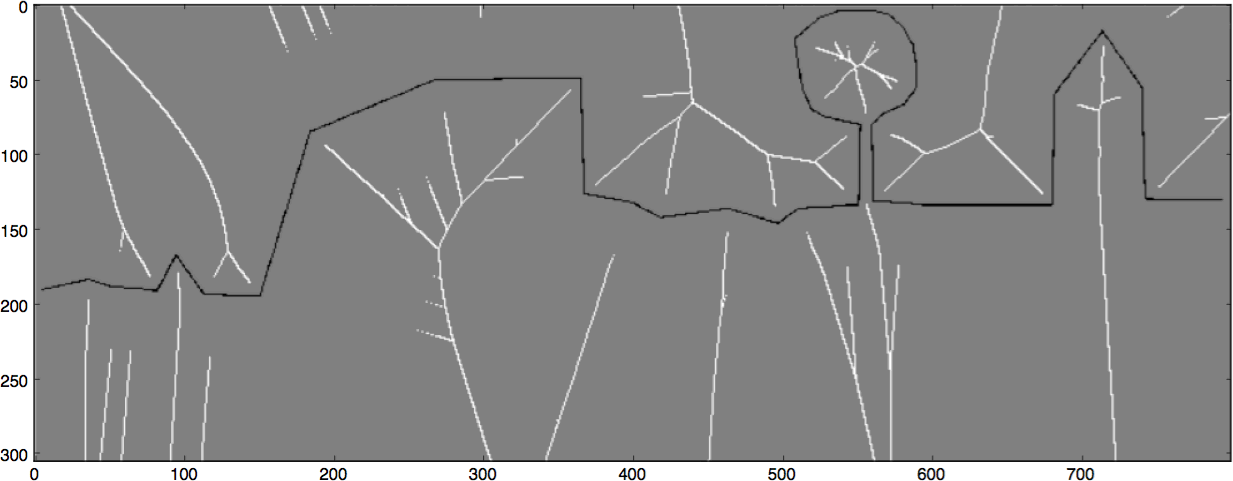
\includegraphics[width=\linewidth]{figs/rasterimpl/simple_dtm-gamma10_earthskel_.png}
		\caption{MAT with strong pruning ($\lambda=10$).}
		\label{fig:imaimp:e}
	\end{subfigure}
	\quad
	\begin{subfigure}{0.4\linewidth}
		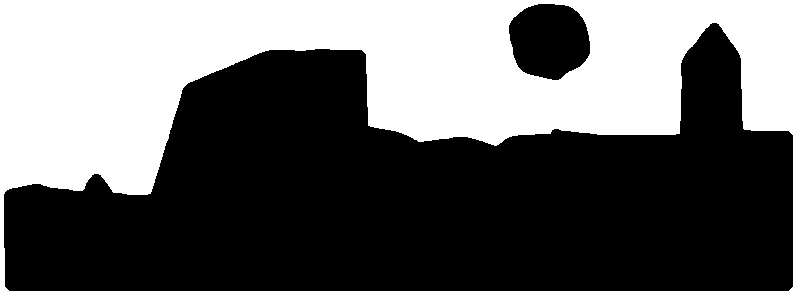
\includegraphics[width=\linewidth]{figs/rasterimpl/simple_dtm-gamma10_earthskel.png}
		\caption{Reconstructed object for $\lambda=10$. Notice how the tree is separated from the the ground and that edges have become rounder.}
		\label{fig:imaimp:f}
	\end{subfigure}
	\caption{The effect of different levels of pruning on the MAT.}
	\label{fig:imaimp}
\end{figure}

% Pruning is virtually always performed as a post-process when the MAT is approximated using a grid method or a method based on the Voronoi Diagram, extremely clean inputs excepted.
% The shrinking ball algorithm, on the other hand, can be modified in such a way that its output does not require pruning afterwards.
% The modification boils down to checking during each iteraions the separation angle of the candidate medial ball.
% When the separation angle drops below a threshold, the algorithm is terminated and the current candidate ball is picked as the definitive medial ball for the current boundary point.
% This is illustrated in Figure~\ref{fig:sb_noise}, \ie\ because the separation angle $\theta_{i+1}$ of the next atom is very small, the shrinking ball process is terminated at the current atom $\mathbf{c_i}$.
% Notice that the separation angle became so small because the candidate feature point `jumped' from one side of the boundary to the other side (compare $\mathbf{q_i}$ and $\mathbf{q_{i+1}}$).
% This typically happens in the presence of noisy boundary points, and illustrates why filtering on a low separation angle is effective for pruning.

\section{Notes and comments}
The Medial Axis Transform was originally introduced in 1967 by Harry Blum, a biologist \citep{Blum67}.

\citet{Ma12} introduced the shrinking ball algorithm. \citet{Peters18} explains how to make the algorithm robust so that it can be successfully applied to lidar point cloud inputs and how to obtain a sheet and cluster segmentation using a region-growing approach.


%%%
%
\section{Exercises}

\begin{enumerate}
  \item Draw the medial axis of a 2D box. Then draw the medial bisectors. How could the medial bisector be used to distinguish between the different sheets?
  \item For what closed object the MAT is a single point?
  \item Do think the MAT could help us to detect thick and thin parts of an object? If so, how?
\end{enumerate}